\documentclass[../../AdvancementSummary.tex]{subfiles}

\begin{document}



%%%%%%%%%%%%%%%%%%%%%%%%%%%%%%%%%%%%%%%%%%%%%%%%%%%
\section{Results: Steric Effects, Stiffening, and Electrostatics}
%%%%%%%%%%%%%%%%%%%%%%%%%%%%%%%%%%%%%%%%%%%%%%%%%%%

%%%%%%%%%%%%%%%%%%%%%%%%%%%%%%%%%%%%%%%%%%%%%%%%%%%
\subsection{Ligand Occlusion}
%%%%%%%%%%%%%%%%%%%%%%%%%%%%%%%%%%%%%%%%%%%%%%%%%%%

Generally, FJCs are most likely to be in a `hairball' conformation. From our simple model of a disordered protein, we may answer some basic questions.  What is the probability that a ligand will be able to bind a specific site on a cytosolic disordered protein?  How does this probability change when the protein is anchored to the membrane?  How do these probabilities change with the contour length of the protein, size of the ligand, and where the binding site is located along the length of the protein?

We can see that in free space, the ligand is more occluded when there are more rods and/or the ligand is larger.  These are both intuitive results. A longer chain creates more conformations where any location on the chain will be occluded by other segments.  A shorter or less flexible chain will not be able to bend enough to bury a binding site.  A larger ligand will require more space near the binding site to be open, which is naturally less likely. A binding site in the middle of the polymer will also be less available to ligand binding since it is more likely sheltered by the rest of the `hairball' polymer. \hl{explain middle better}

In half space, the polymer has fewer conformations it can take on since it can only occupy half of the region. This prevents many more `hairball' conformations than it prevents straightened conformations.  Overall, the effect is an overall straightening of the polymer in the presence of a membrane. 

\begin{figure}[h]
	\begin{center}
		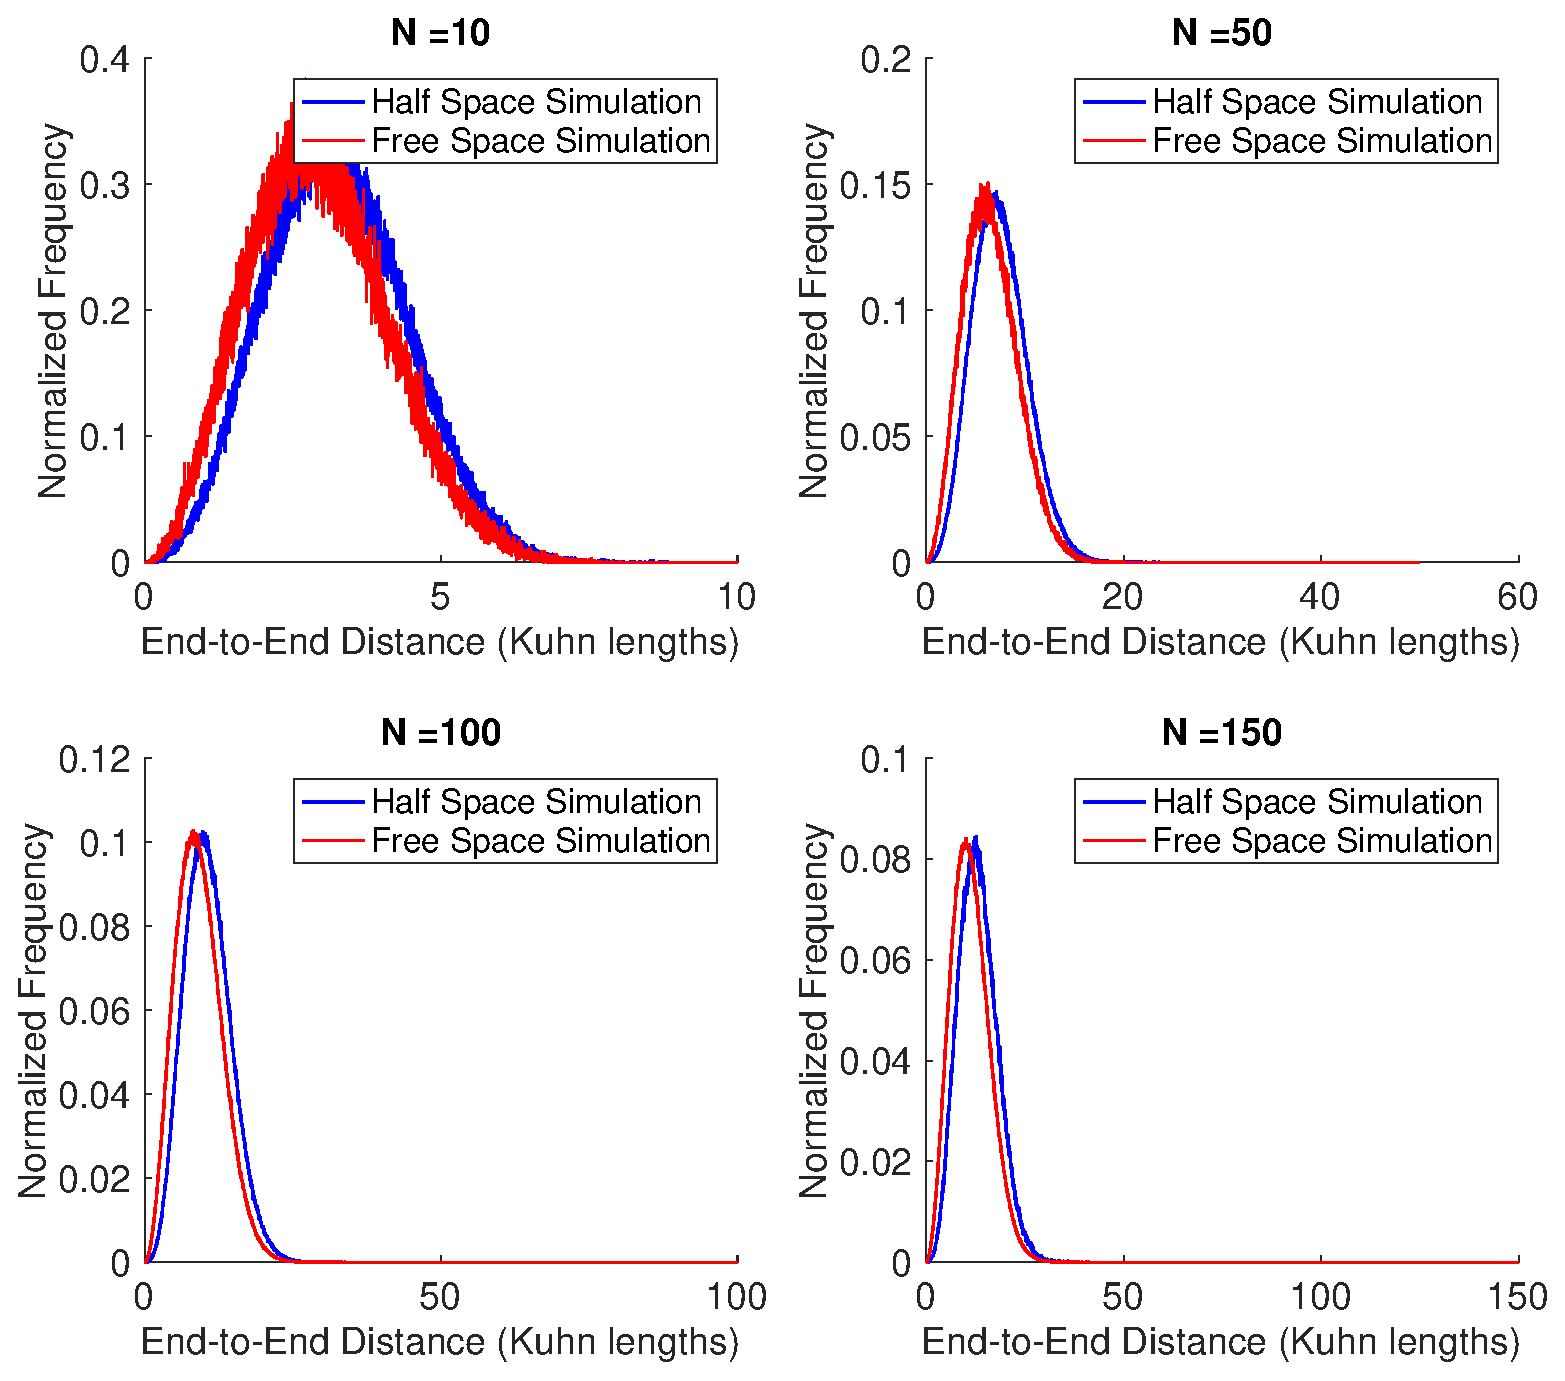
\includegraphics[width=0.8\linewidth]{ResultsFigures/General/ReeDistributionHalfVSFreeSim.eps}
		\caption{Distributions of polymer end-to-end distance in free space and half space for various polymer lengths (N). For each length, the end-to-end distance of the polymer in half-space is overall straighter than in free space.}
	\end{center}
\end{figure}


The membrane increases the likelihood of straighter conformations, which would be likely to increase the binding probability. However, the membrane itself may also occlude the ligand since we include an orientation of the binding site in our simulation. Therefore if the binding site is oriented down towards the membrane, then even if the polymer is not occluding the ligand, the membrane still might. When we include a hard plane membrane in our simulation, we see that the presence of a membrane generally decreases the probability of ligand binding.  When the ligand is small enough, the difference in binding probabilities between free space and half space binding is minimal.

\hl{Re-bin histograms} \hl{Include image of simulation?  Usually look bad....but might be a worthwhile visual.}
\hl{This is really ugly.}
\hl{Accidentally omitted last column?}
\hl{Color bars need to be fixed to be consistent somehow}
\hl{Color scales the same?}


\begin{figure}[H]
\begin{center}
\begin{subfigure}{0.4\linewidth}
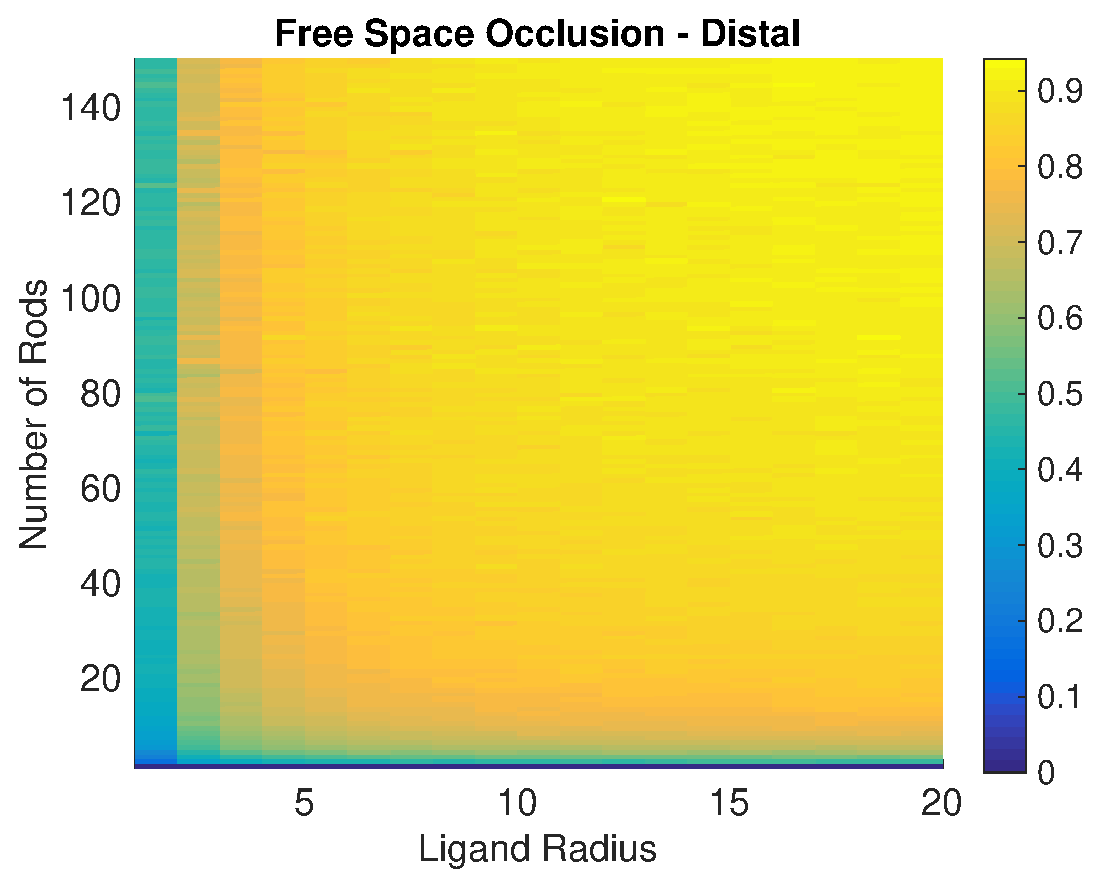
\includegraphics[width=\linewidth]{ResultsFigures/General/OcclusionVSNVSRFree.eps}
\caption{}
\end{subfigure}
\begin{subfigure}{0.4\linewidth}
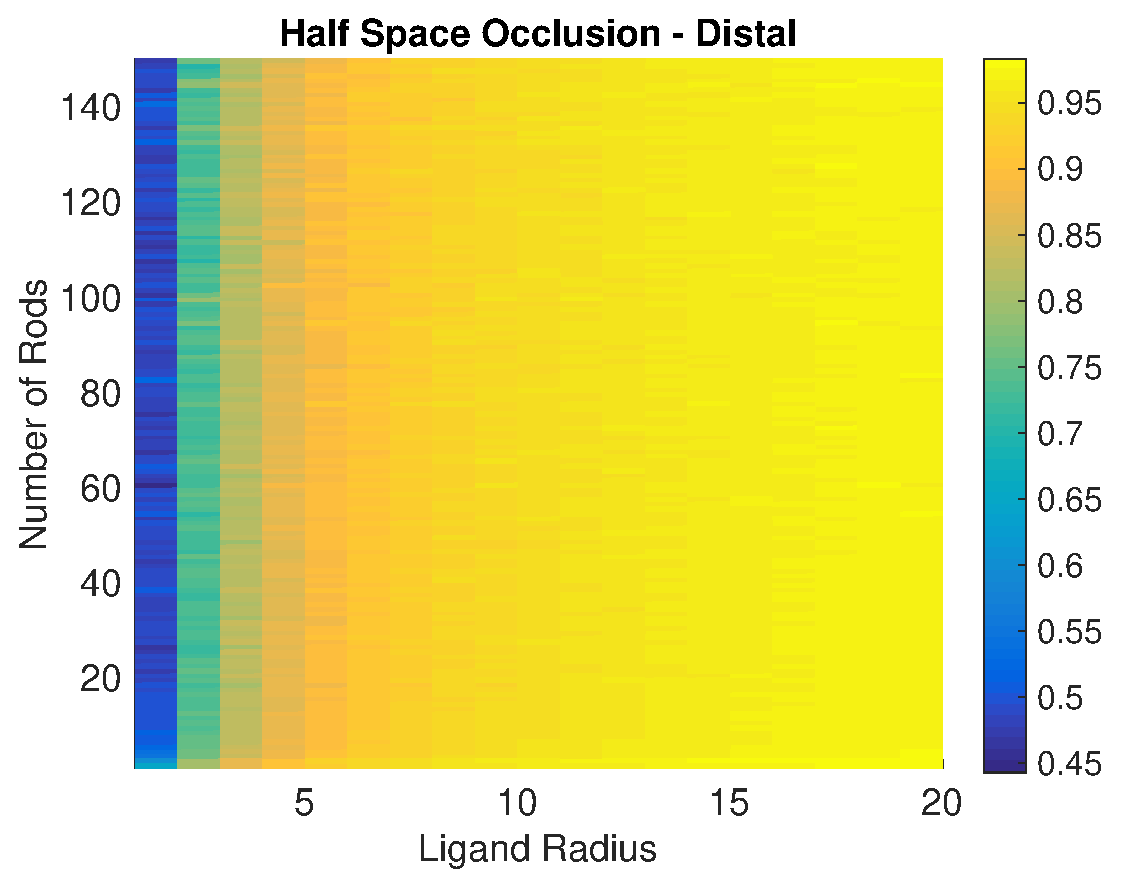
\includegraphics[width=\linewidth]{ResultsFigures/General/OcclusionVSNVSRHalf.eps}
\caption{}
\end{subfigure}
\begin{subfigure}{0.4\linewidth}
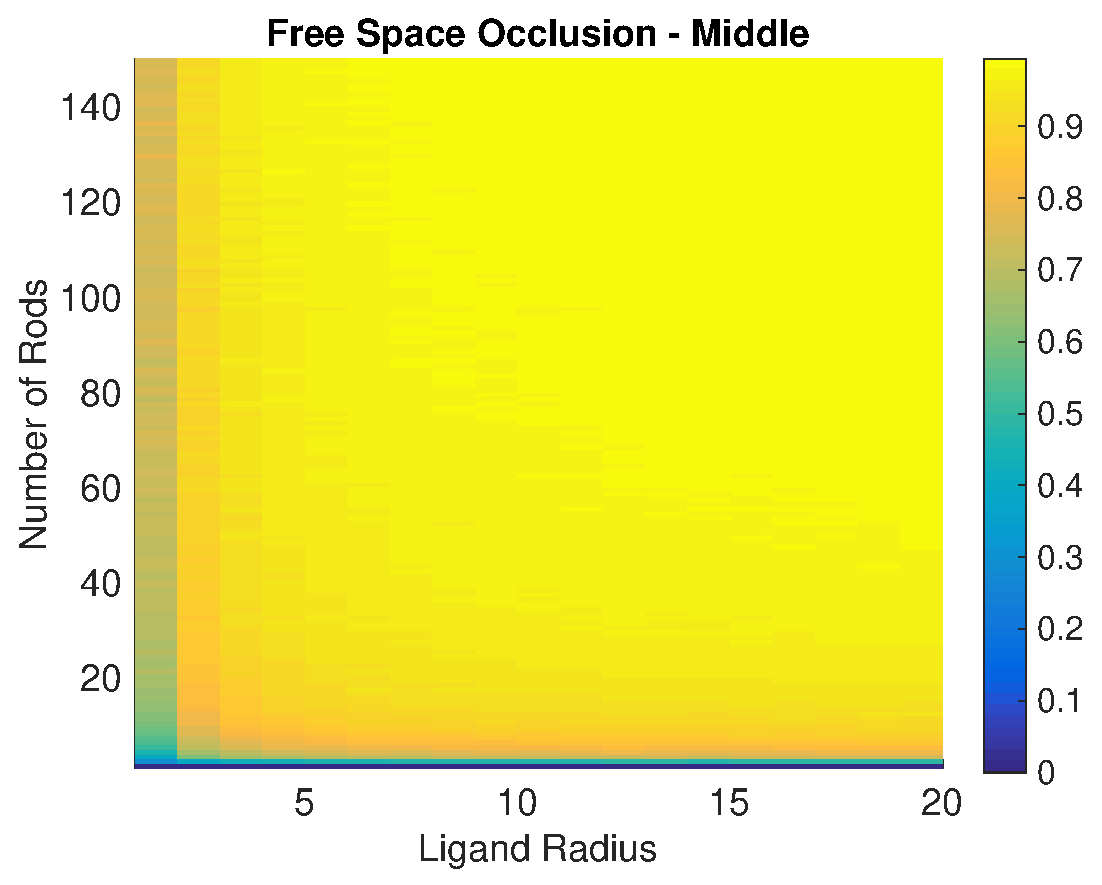
\includegraphics[width=\linewidth]{ResultsFigures/General/OcclusionVSNVSRFreeMid.eps}
\caption{}
\end{subfigure}
\begin{subfigure}{0.4\linewidth}
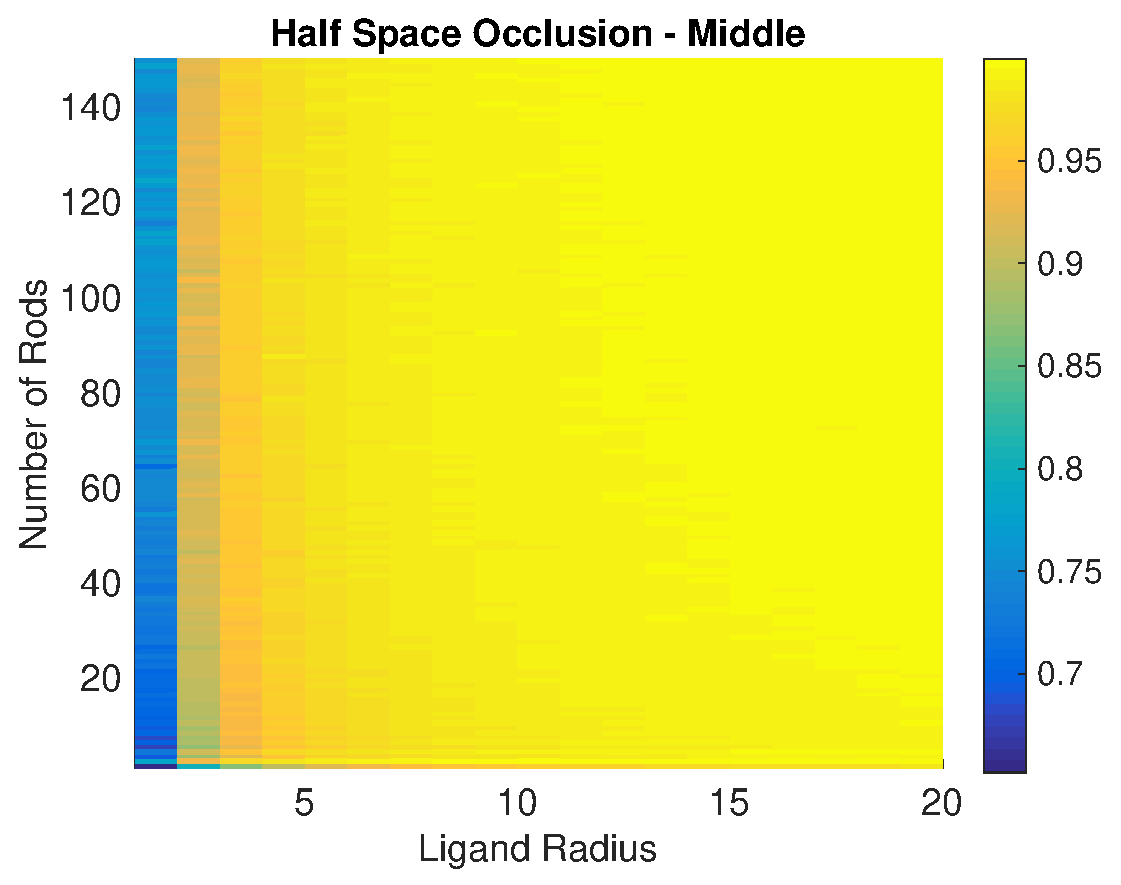
\includegraphics[width=\linewidth]{ResultsFigures/General/OcclusionVSNVSRHalfMid.eps}
\caption{}
\end{subfigure}
\caption{Probability of occluding a ligand of variable radius from a polymer of variable contour length when the binding site is at the distal end or middle of the chain in free space or half space. (a) Free space polymer with binding site at distal end. (b) Half space polymer with binding site at distal end. (c) Free space polymer with binding site in the middle. (d) Half space polymer with binding site in the middle.}
\end{center}
\end{figure}

%%%%%%%%%%%%%%%%%%%%%%%%%%%%%%%%%%%%%%%%%%%%%%%%%%%
\subsection{Disorder-to-Order Transitions}
%%%%%%%%%%%%%%%%%%%%%%%%%%%%%%%%%%%%%%%%%%%%%%%%%%%

\subsubsection{Introduction}

Intrinsically disordered proteins sterically occlude ligands by transiently sequestering the binding site. There is evidence that indicates some IDPs undergo a disordered-to-ordered transition upon post-translational modification, i.e. phosphorylation. For example, phosphorylation of PAGE4 restricts the number of conformations it may explore, increasing rigidity of the backbone.\cite{He2015} Post-translational modifications may also cause a conformational change, altering the availability of the binding site.  The neural protein 4E-BP2 undergoes multisite phosphorylation which leads to a disorder-to-order transition, forming $\beta$ sheets which hide the eIF4E binding site. \cite{Bah2015} \hl{Any other examples to include?}

We are interested in how cooperative effects may arise in reactions with a disordered protein. One model we explore is disorder-to-order transitions as a result of post-translational modifications. With regards to our case study, CD3$\zeta$, we assume that each phosphorylation event causes a fraction of the chain to undergo a disorder-to-order transition. We investigate how this local structuring phenomenon would impact subsequent phosphorylations by Lck along TCR CD3$\zeta$.

\begin{figure}[H]
\begin{center}
    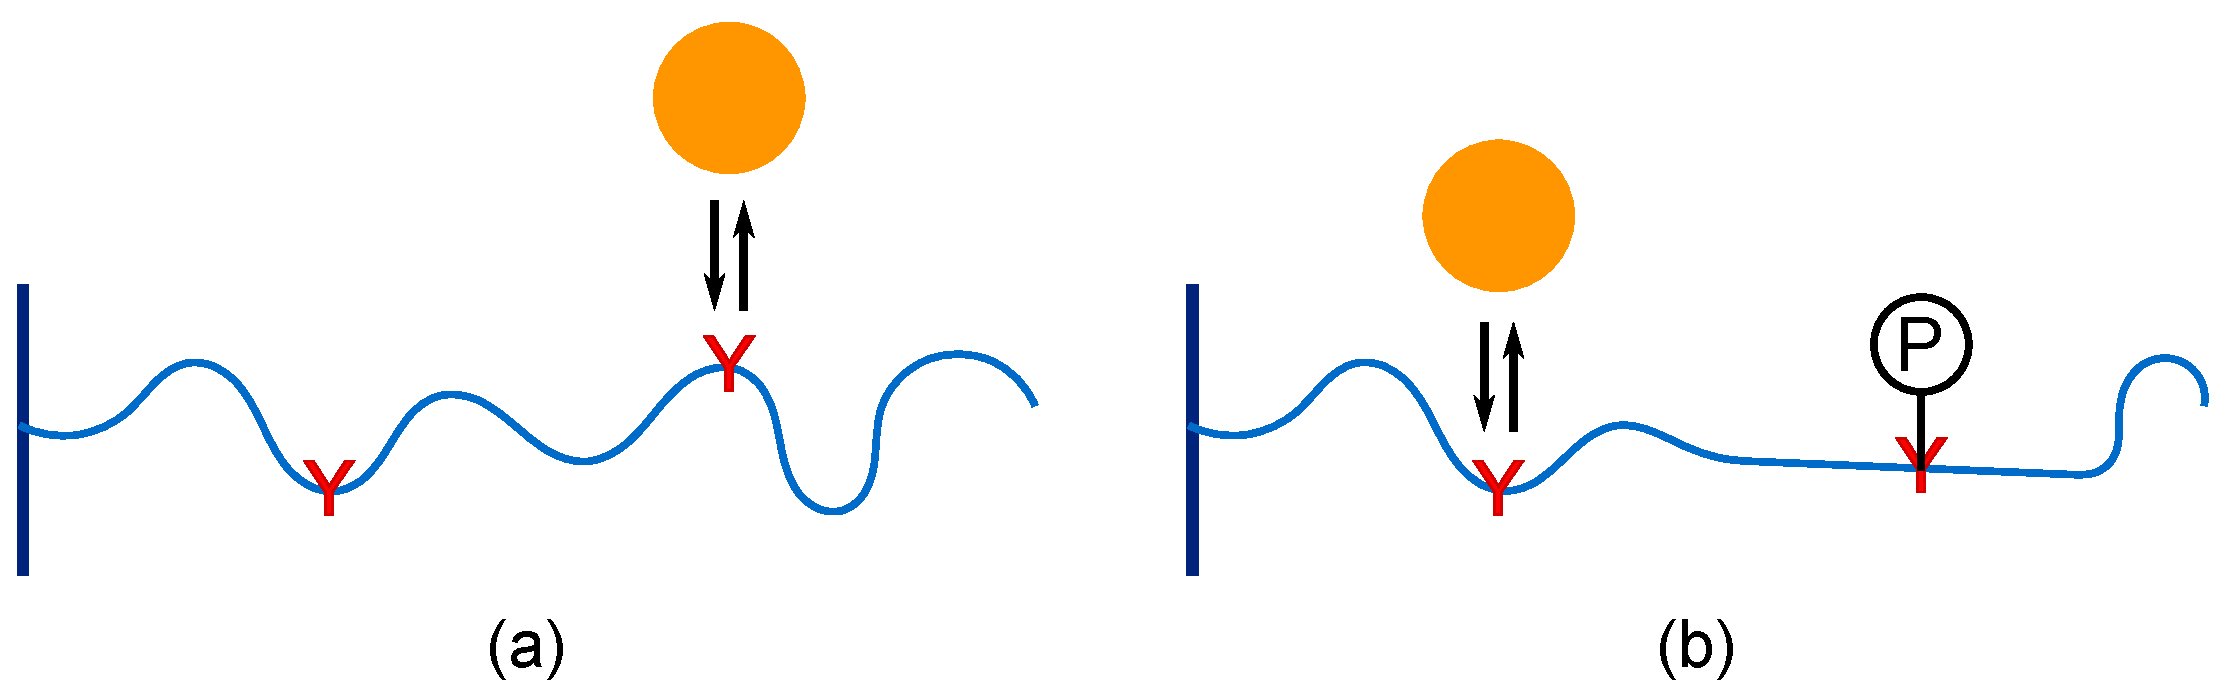
\includegraphics[width=0.8\linewidth]{ResultsFigures/StiffeningDiagram/StiffeningDiagram.eps}
    \caption{Cartoon of partial stiffening model. Entirely floppy FJC prior to modification (a) transitions to partially rigid chain after modification (b).}
    \end{center}
\end{figure}

\subsubsection{Model Modifications}

We include local structuring as a limitation on which joints of the freely jointed chain are allowed to rotate. For each modified residue, some number of joints are effectively frozen in a straight conformation. The number of joints frozen per modification is a parameter we explore. This method of local structuring leaves the original binding site in a primarily available configuration, however, we are interested in how it impacts the neighboring modification targets (i.e. tyrosines to be phosphorylated)


\subsubsection{Cooperativity may arise from local structuring in intrinsically disordered proteins}

If we assume that phosphorylation of tyrosines on the CD3$\zeta$ chain induces local structuring, then neighboring tyrosines will feel a reduction of entropic occlusion.  This will cause them to be more available to binding by a ligand. The magnitude of this effect will vary based on how much structuring occurs, e.g. if it affects the nearest two residues or the nearest ten residues. 

We see from these simulations that the average binding rate of a ligand to the unphosphorylated tyrosines increases as the number of phosphorylated tyrosines (and therefore the number of structured residues) increases. From the first to the sixth phosphorylation event, there is a 3-10 fold increase in the average binding rate for moderate (1/12 of chain length) to severe (1/6 of chain length) local stiffening per phosphorylation.

\hl{We have 10 fold change.  Where does Omer's 100 fold change come in?}

\begin{figure}[H]
	\begin{center}
		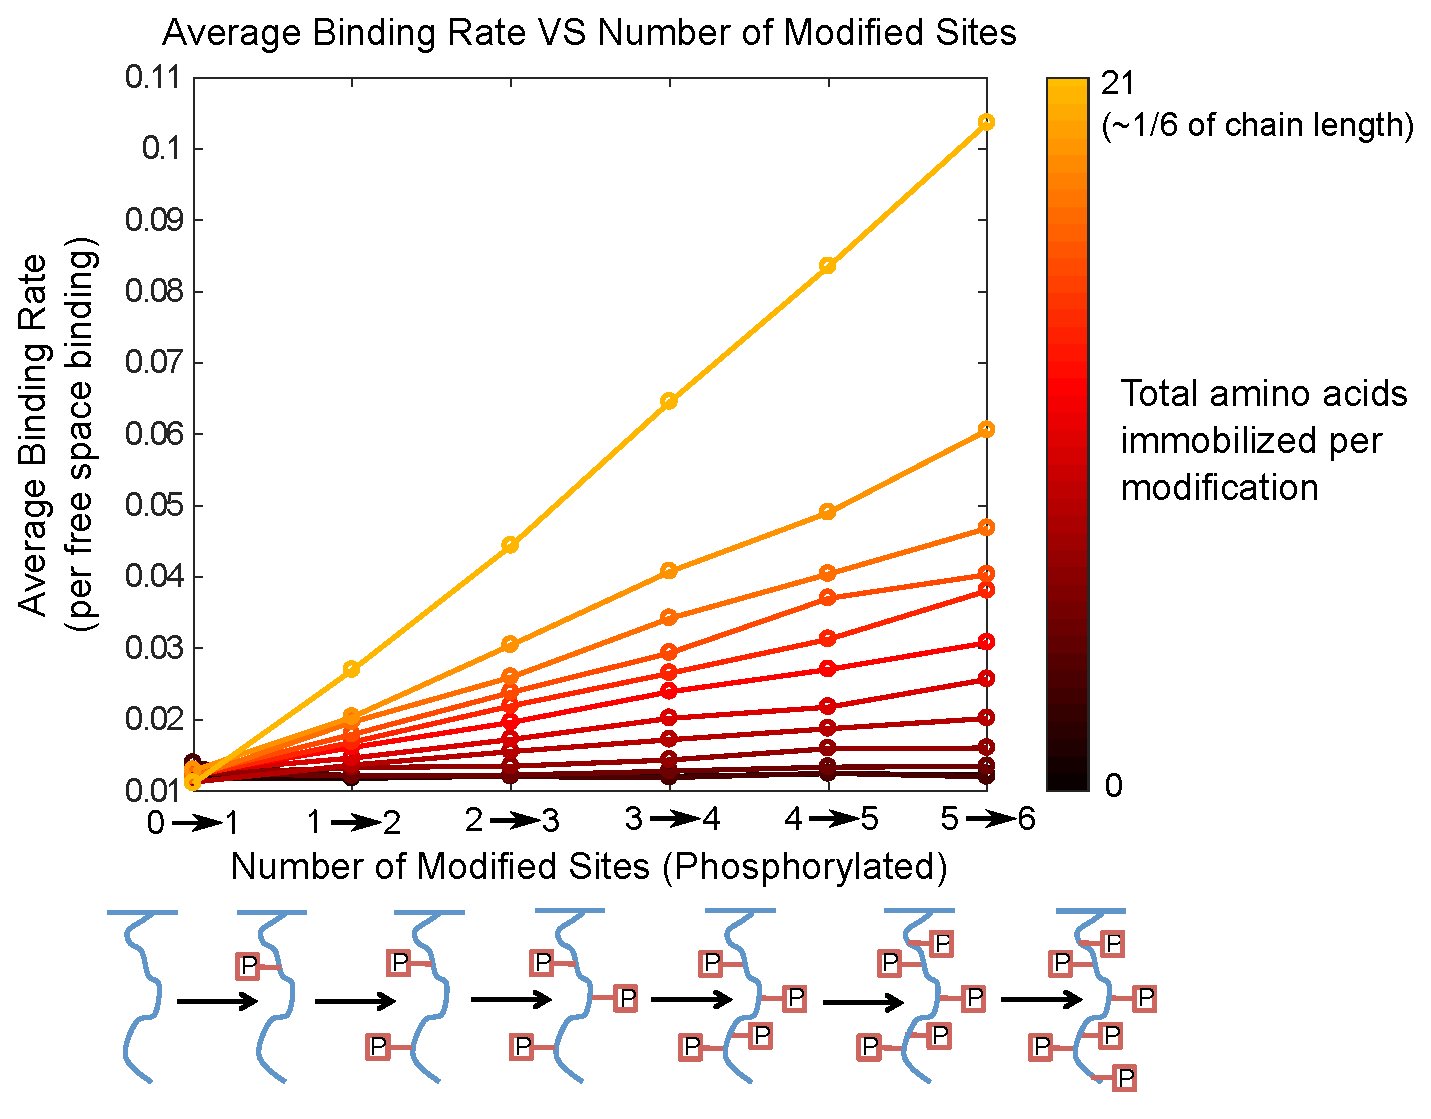
\includegraphics[width=0.8\linewidth]{ResultsFigures/CD3ZetaStiffeningMembraneOn/AvgBindVSTotalPhosColorMapLabeled.eps}
		\caption{(Above) Simulated average binding rates of Lck to CD3$\zeta$ for different levels of phosphorylation given a specified degree of local structuring (none $\rightarrow$ black, low $\rightarrow$ red, high $\rightarrow$ orange). (Below) Cartoon representing a possible phosphorylation state series of CD3$\zeta$. }
	\end{center}
\end{figure}


Local disordered-to-ordered transitions are sufficient to create positive cooperativity of PTMs. Positive cooperativity can increase the sensitivity of a response to changes in ligand concentration and increase the potency of signaling responses.

\hl{Paragraph about benefits?  or is that for discussion?}
\hl{Paragraph about dephosphorylation}

\begin{figure}[H]
	\begin{center}
		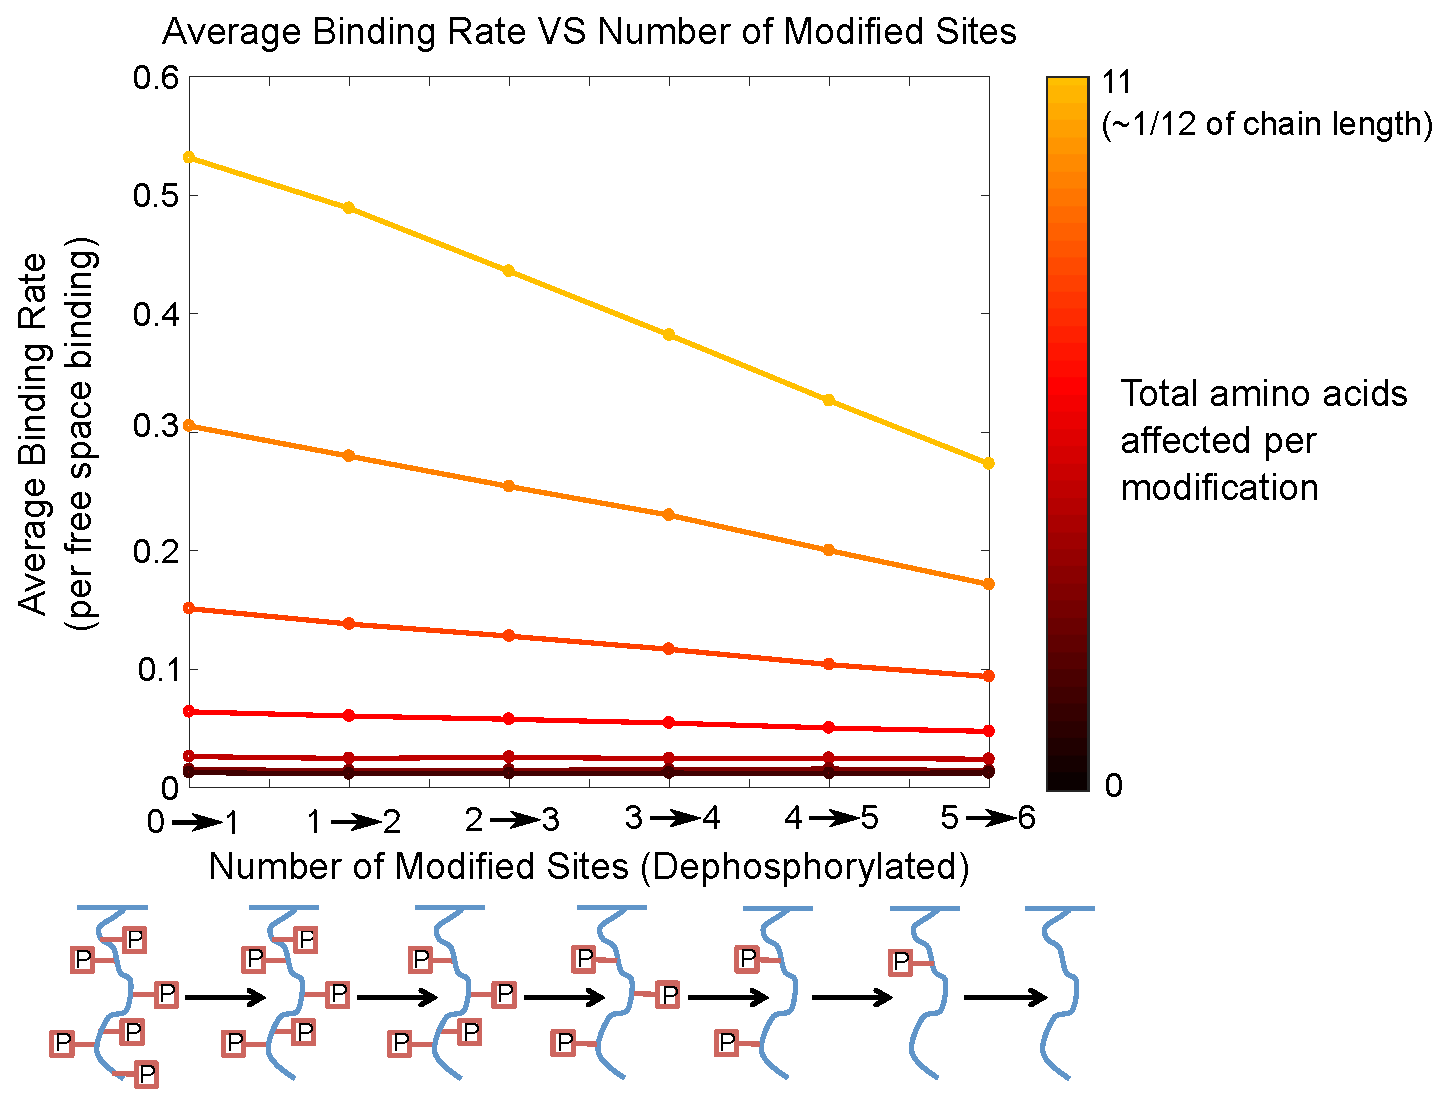
\includegraphics[width=0.8\linewidth]{ResultsFigures/CD3ZetaStiffeningMembraneOn/Dephosphorylation/AvgBindVSTotalModified5.eps}
		\caption{(Above) Simulated average binding rates of Lck to CD3$\zeta$ for different levels of dephosphorylation given a specified degree of local unstructuring (none $\rightarrow$ black, low $\rightarrow$ red, high $\rightarrow$ orange).}
	\end{center}
\end{figure}




\subsubsection{Future Work}

We will explore dephosphorylation/unstructuring of a fully rigid disordered protein. 

We will create Hill curves of phosphorylation, dephosphorylation, and reversible phosphorylation.  This will allow us to better understand and communicate our results with the rest of the biochemistry commmunity. In particular, the Hill curve of reversible phosphorylation will indicate if ultrasensitivity is achievable through this mechanism. \hl{true?}

\subsubsection{Sequential Binding}

We hypothesized that without any modifications due to binding, then with only the presence of a membrane, we would see preferential binding in an outwards to inwards (6-5-4-3-2-1) manner.  In regards to our model system, that is to say we expected the tyrosine furthest from the membrane to be phosphorylated first and the tyrosine closest to the membrane to be phosphorylated last.  We surmised this from the idea that tyrosine's too close to the membrane would see extra kinase inhibition from membrane occlusion, whereas the tail of the disordered protein would not experience this same effect. 

When considering the partial stiffening model, we predict that this effect would be enhanced.  In an unphosphorylated state, if the tyrosine furthest from the membrane is most likely to be bound, then partial stiffening would give increased preference to the next furthest from the membrane (here called the fifth tyrosine) as the second to be phosphorylated.  This comes from the reduction of total configurations available to the protein.  Since the stiffening would occur around the sixth tyrosine, the nearest unphosphorylated tyrosine would be the most affected.  The segment of polymer near the fifth tyrosine would have fewer available conformations and therefore proportionately fewer would be occluding the fifth tyrosine.

\hl{Explain the above better.  Not totally convinced that's the best argument.  What's the correct term for 'unoccluded'?  Available?  Open?}

\hl{Do we introduce this as a purposeful topic or as a neat thing that falls out?  Include Dushek paper as benefit or as intro?}

We obtained relative probabilities of binding for each tyrosine along the chain at each phosphorylation state.  With this information, we are able to explore whether or not there is a dominant sequence of phosphorylation events. We ran a Gillespie algorithm with six events, one for each phosphorylation.  From each run, we record which sequence or 'path' of phosphorylation.  When we compile the path frequency data, it becomes clear that the first phosphorylation event is dominant.  That is to say, any path beginning by phosphorylating the membrane distal tyrosine (6th tyrosine), will occur more often than any path beginning with the membrane proximal tyrosine. 

For simplicity, we consider only the paths membrane proximal to membrane distal (123456) and distal to proximal (654321). We see that when a membrane is present, the probability of phosphorylating distal to proximal is much higher than that of phosphorylating proximal to distal.  It is also more probable than if all paths were equally likely. This phenomenon is easily explained by the presence of a membrane. The membrane proximal tyrosine has a smaller range of space it may occupy than the distal tyrosine.  Therefore, it is more likely to be close to the membrane in a configuration.  Since the ligand cannot penetrate the membrane, tyrosines closer to the membrane have a higher probability of being effectively sheltered from ligand binding. This makes the distal to proximal path much more likely, regardless of local stiffening effects. This path preference is enhanced with local structuring since the distal tyrosine is more accessible and local structuring makes neighboring tyrosines even more available.

One would expect then, that a cytoplasmic disordered protein would not experience a path preference between N-terminal to C-terminal or vice versa. When we simulate CD3$\zeta$ without a membrane, there is still a marked preference for C-terminal to N-terminal phosphorylation.  This effect arises from the spacing of the tyrosines along the polymer's length.  \hl{As we noted above,} the location of a tyrosine impacts how likely a ligand is to bind there. Since the tyrosines in CD3$\zeta$ are not equally spaced along the length of the protein, there is a bias for the tyrosine closest to one end, in this case the tyrosine closest to the C-terminal. When we simulate a polymer with the same length as CD3$\zeta$ but equally spaced tyrosines, we see that there is no longer a preference between the two paths. 



We are soon going to introduce a ranking system for the paths in order to do a full analysis of all possible paths. This will help analyze the likelihood of any of the non-sequential paths.

\hl{Better to make one figure and label a,b,c in Inkscape?}

\begin{figure}[H]
	\begin{center}
		\begin{subfigure}{0.3\linewidth}
			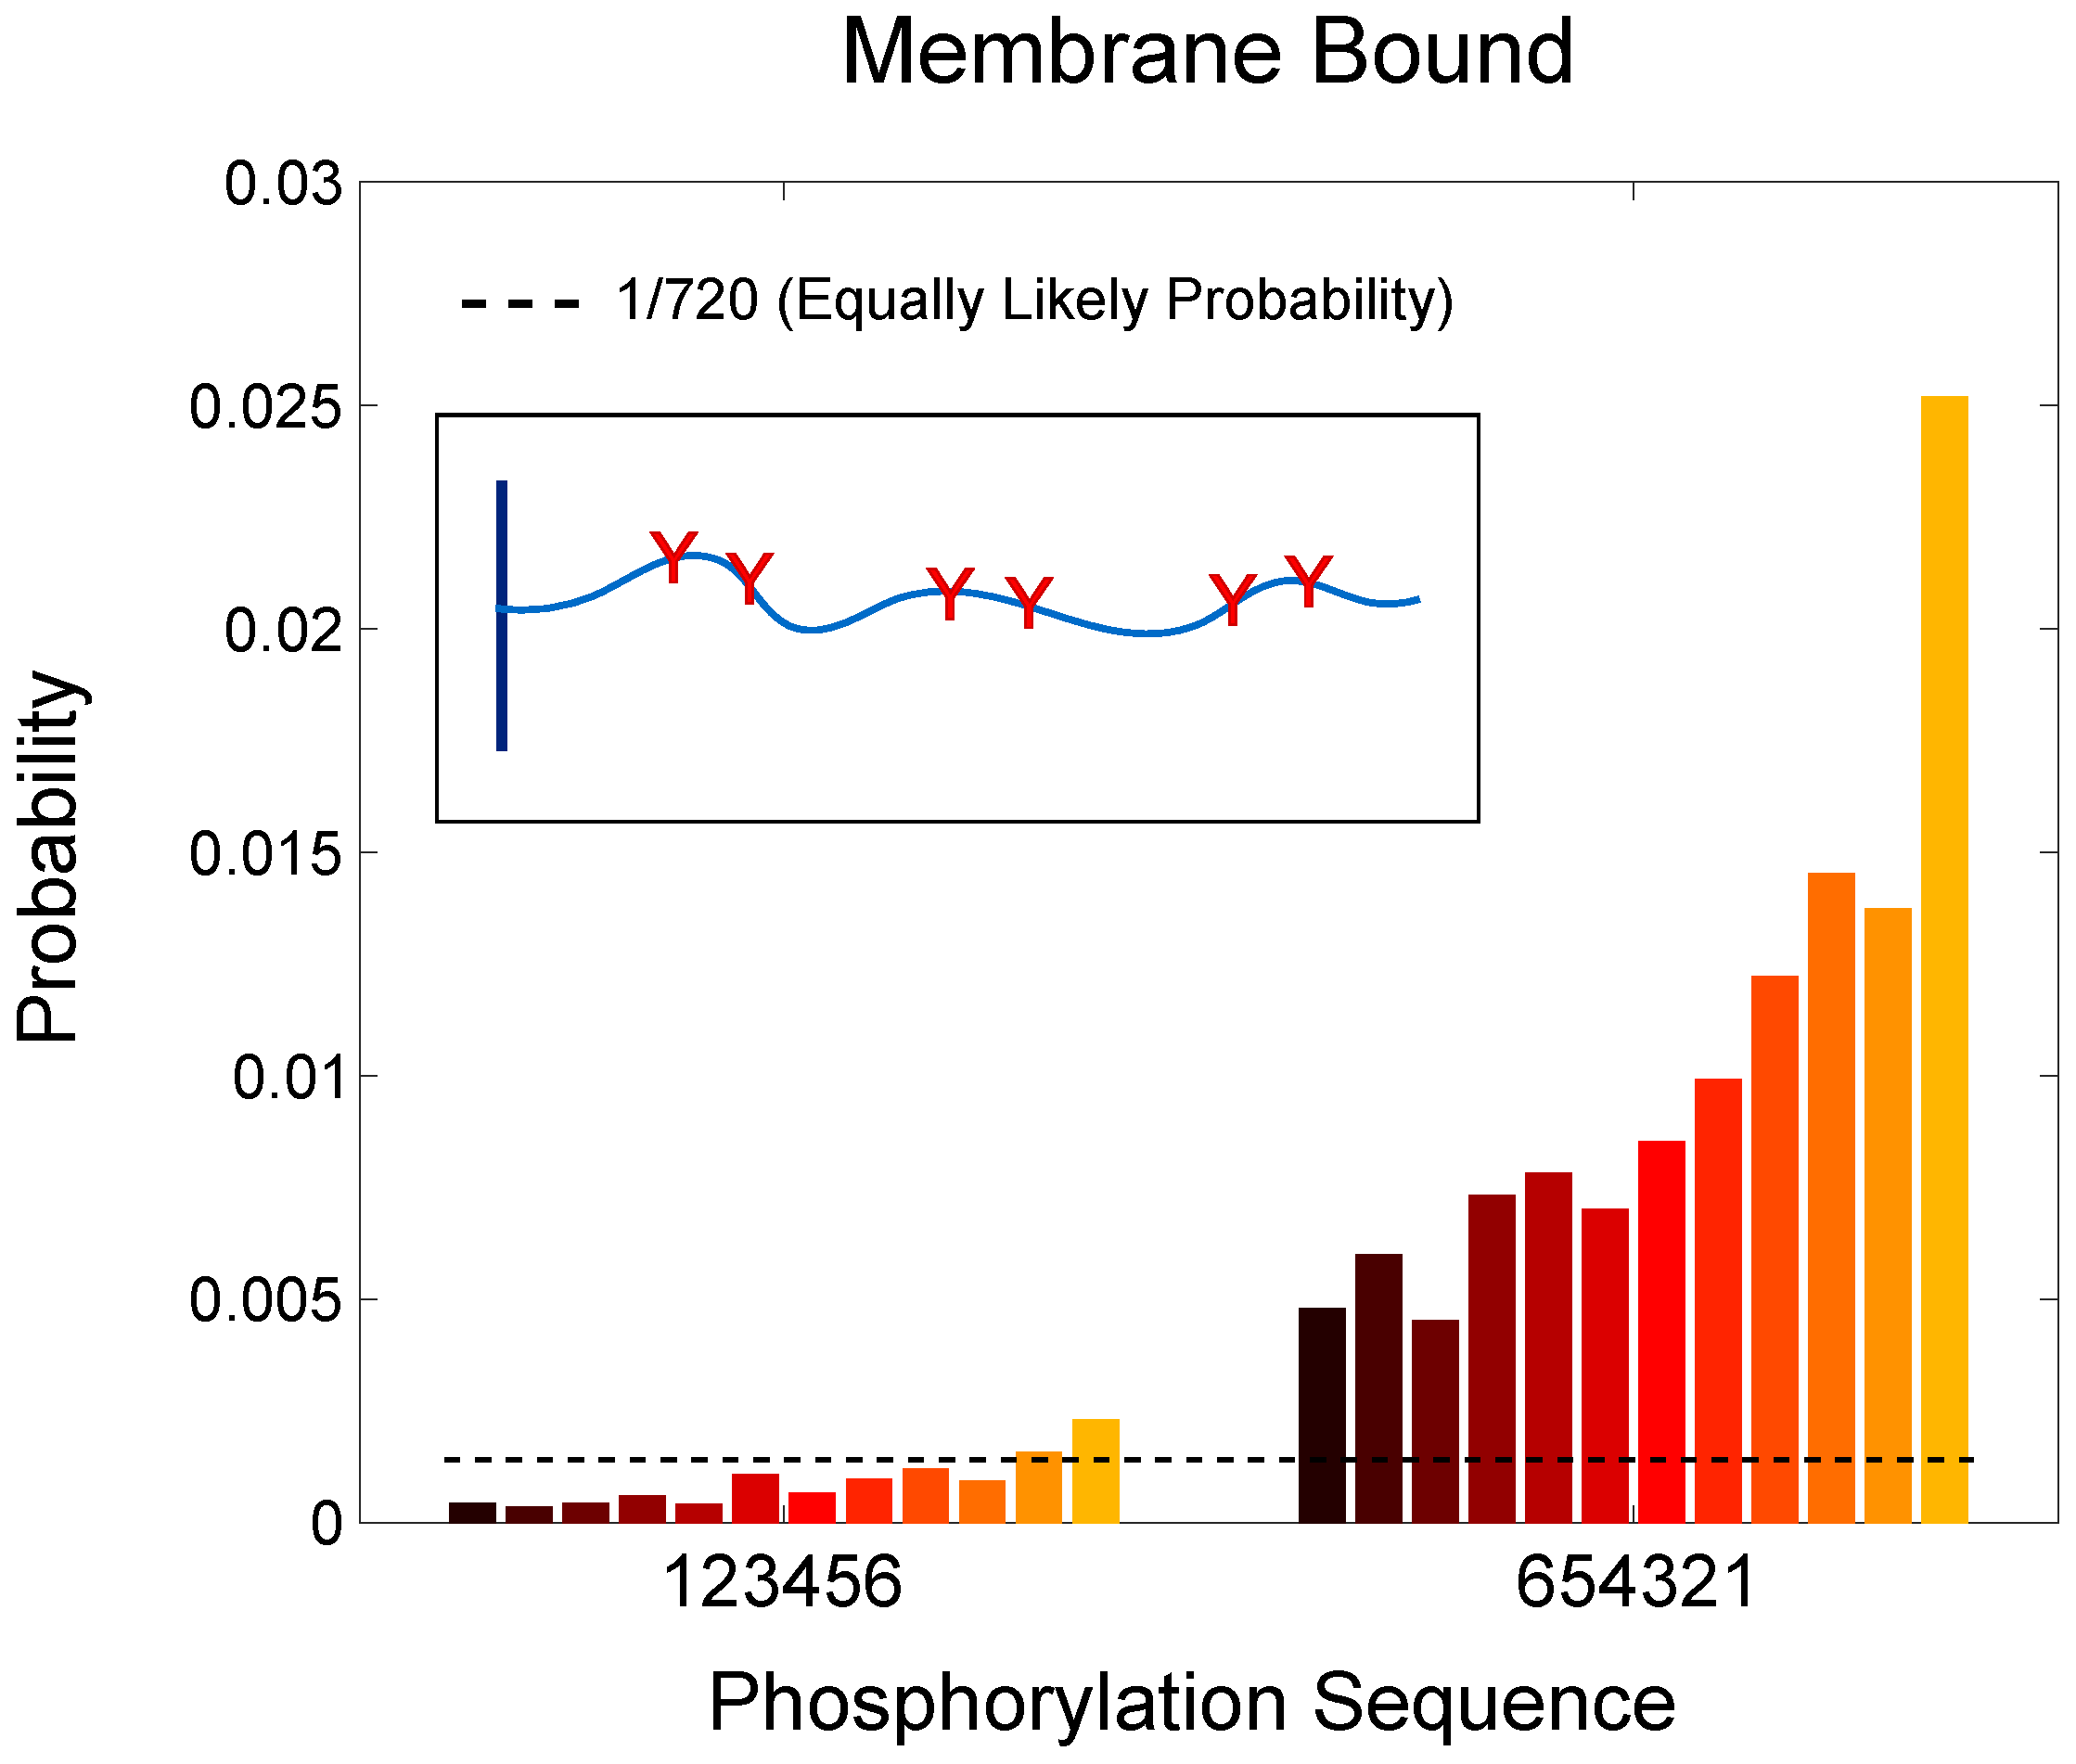
\includegraphics[width=\linewidth]{ResultsFigures/StiffeningSequentialBinding/MemOn/ProbVSSequence.eps}
			\caption{}
		\end{subfigure}
		\begin{subfigure}{0.3\linewidth}
			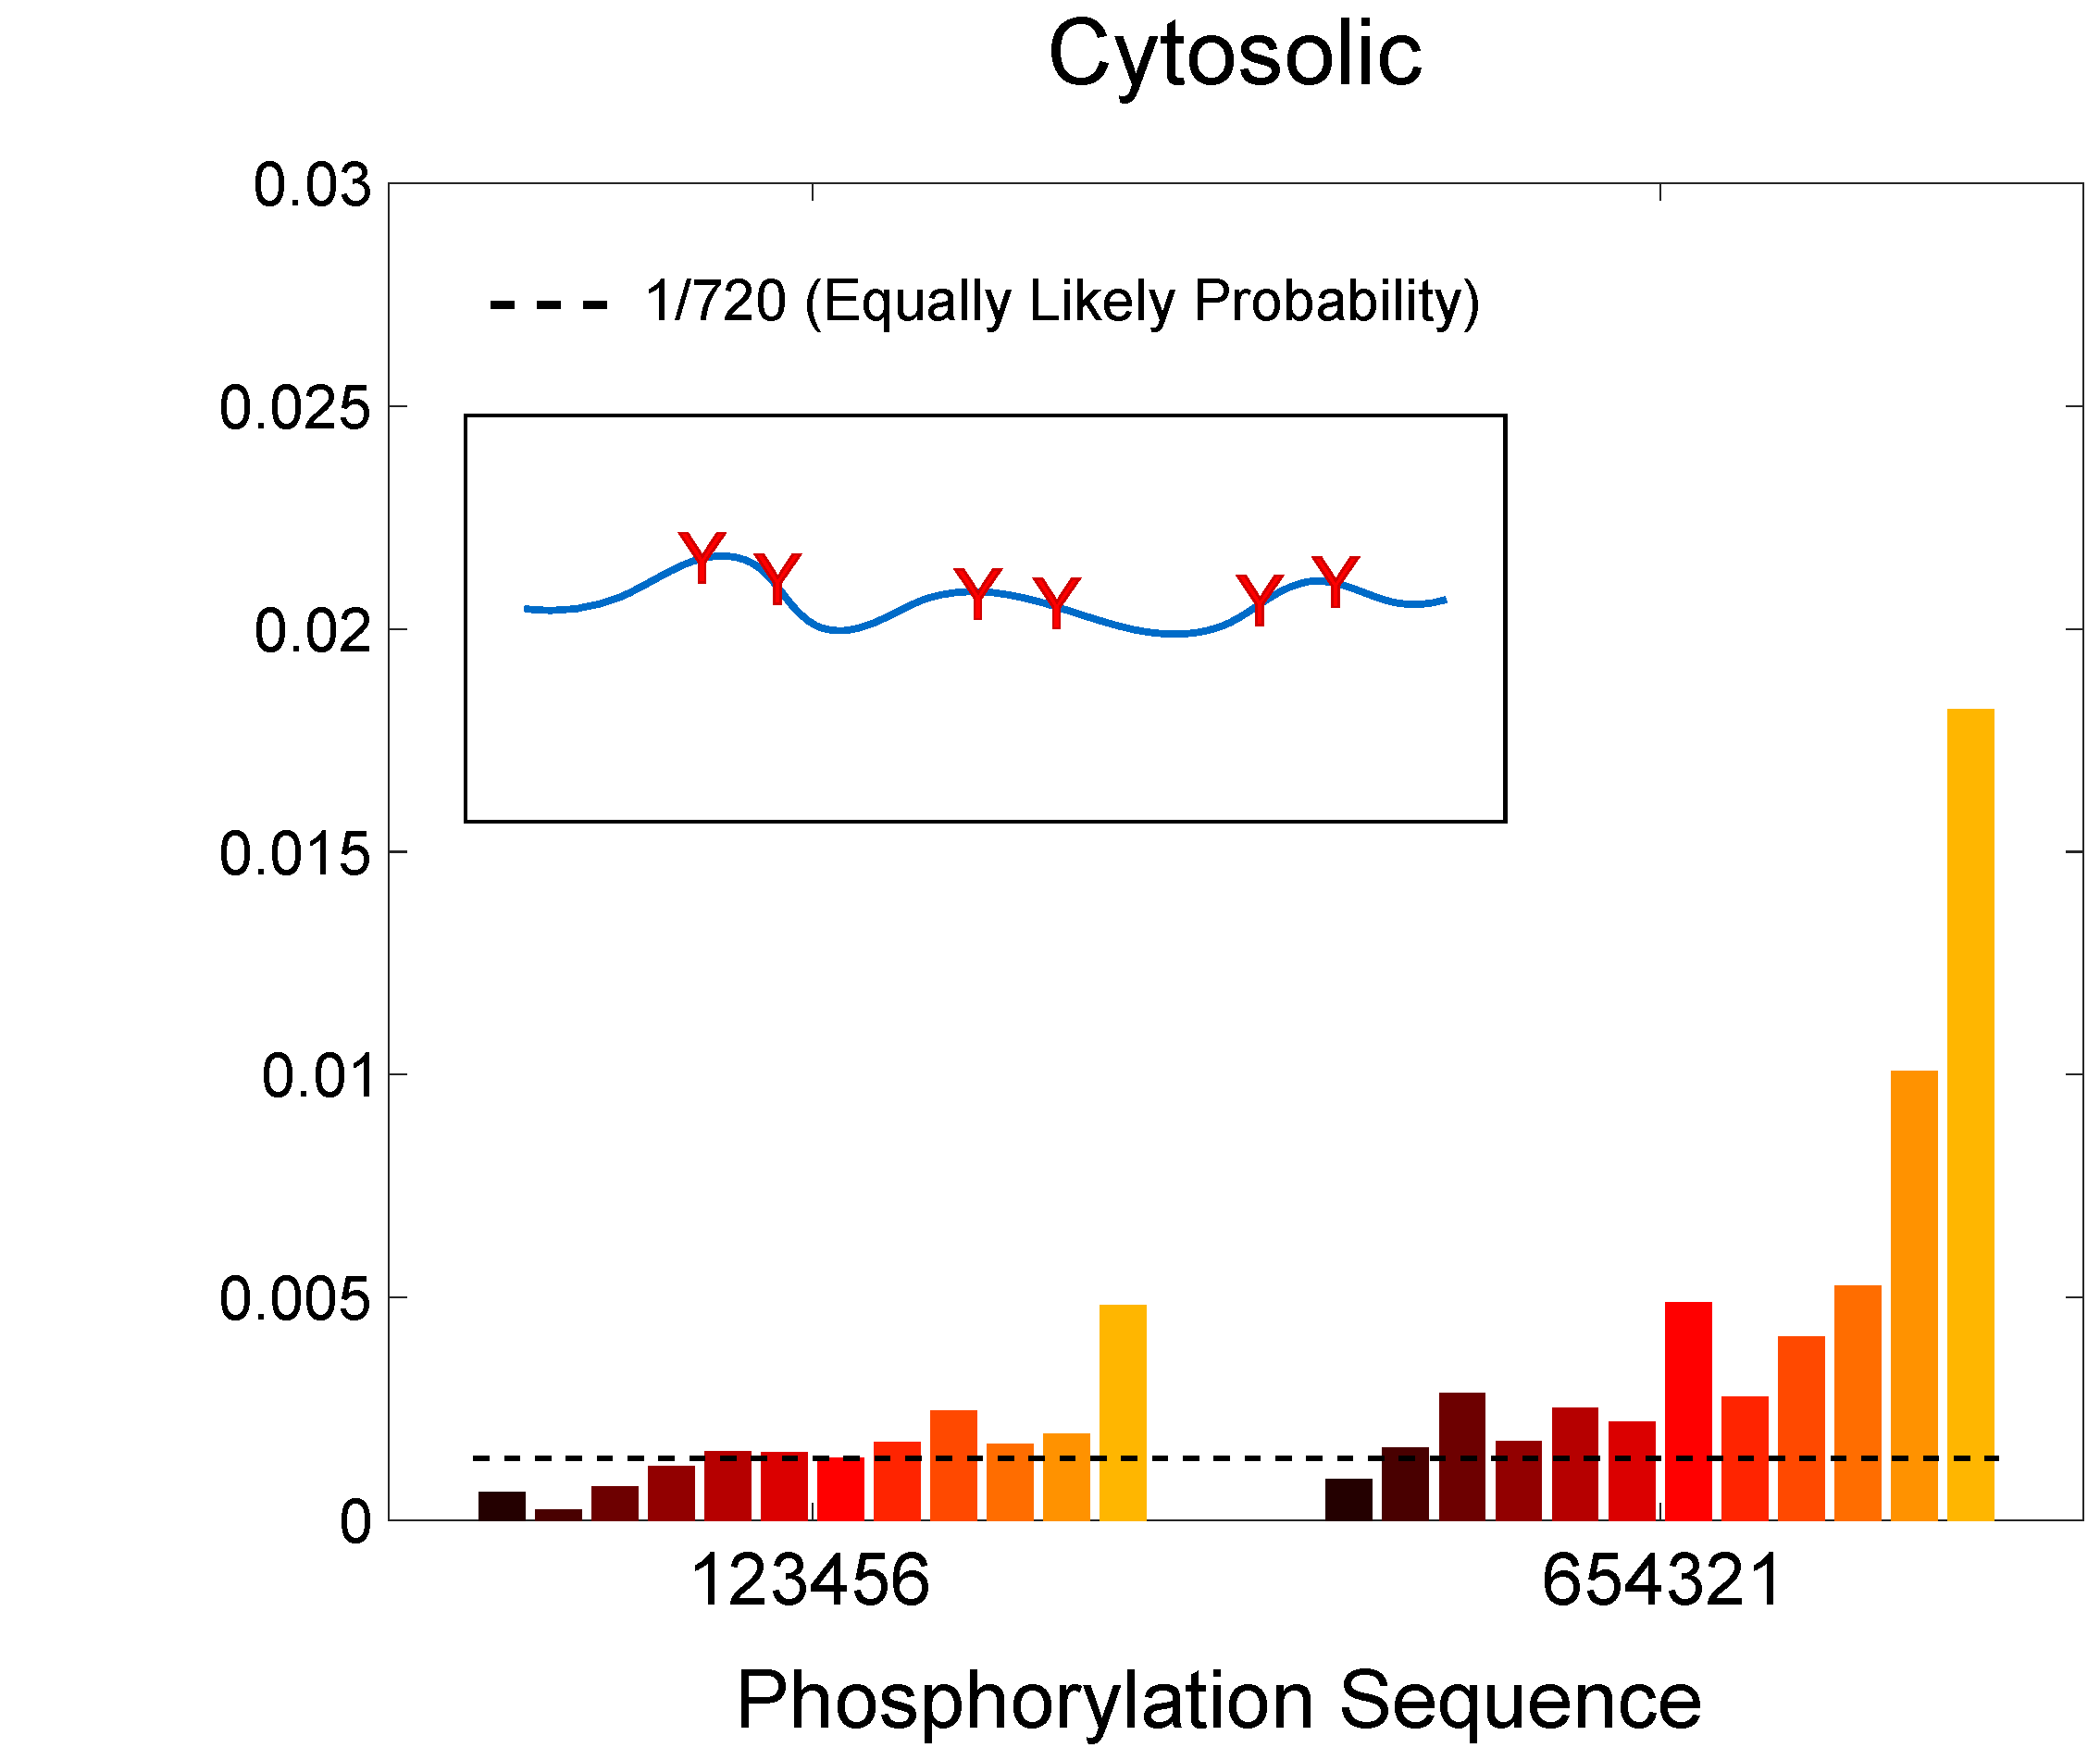
\includegraphics[width=\linewidth]{ResultsFigures/StiffeningSequentialBinding/MemOff/ProbVSSequence.eps}
			\caption{}
		\end{subfigure}
		\begin{subfigure}{0.3\linewidth}
			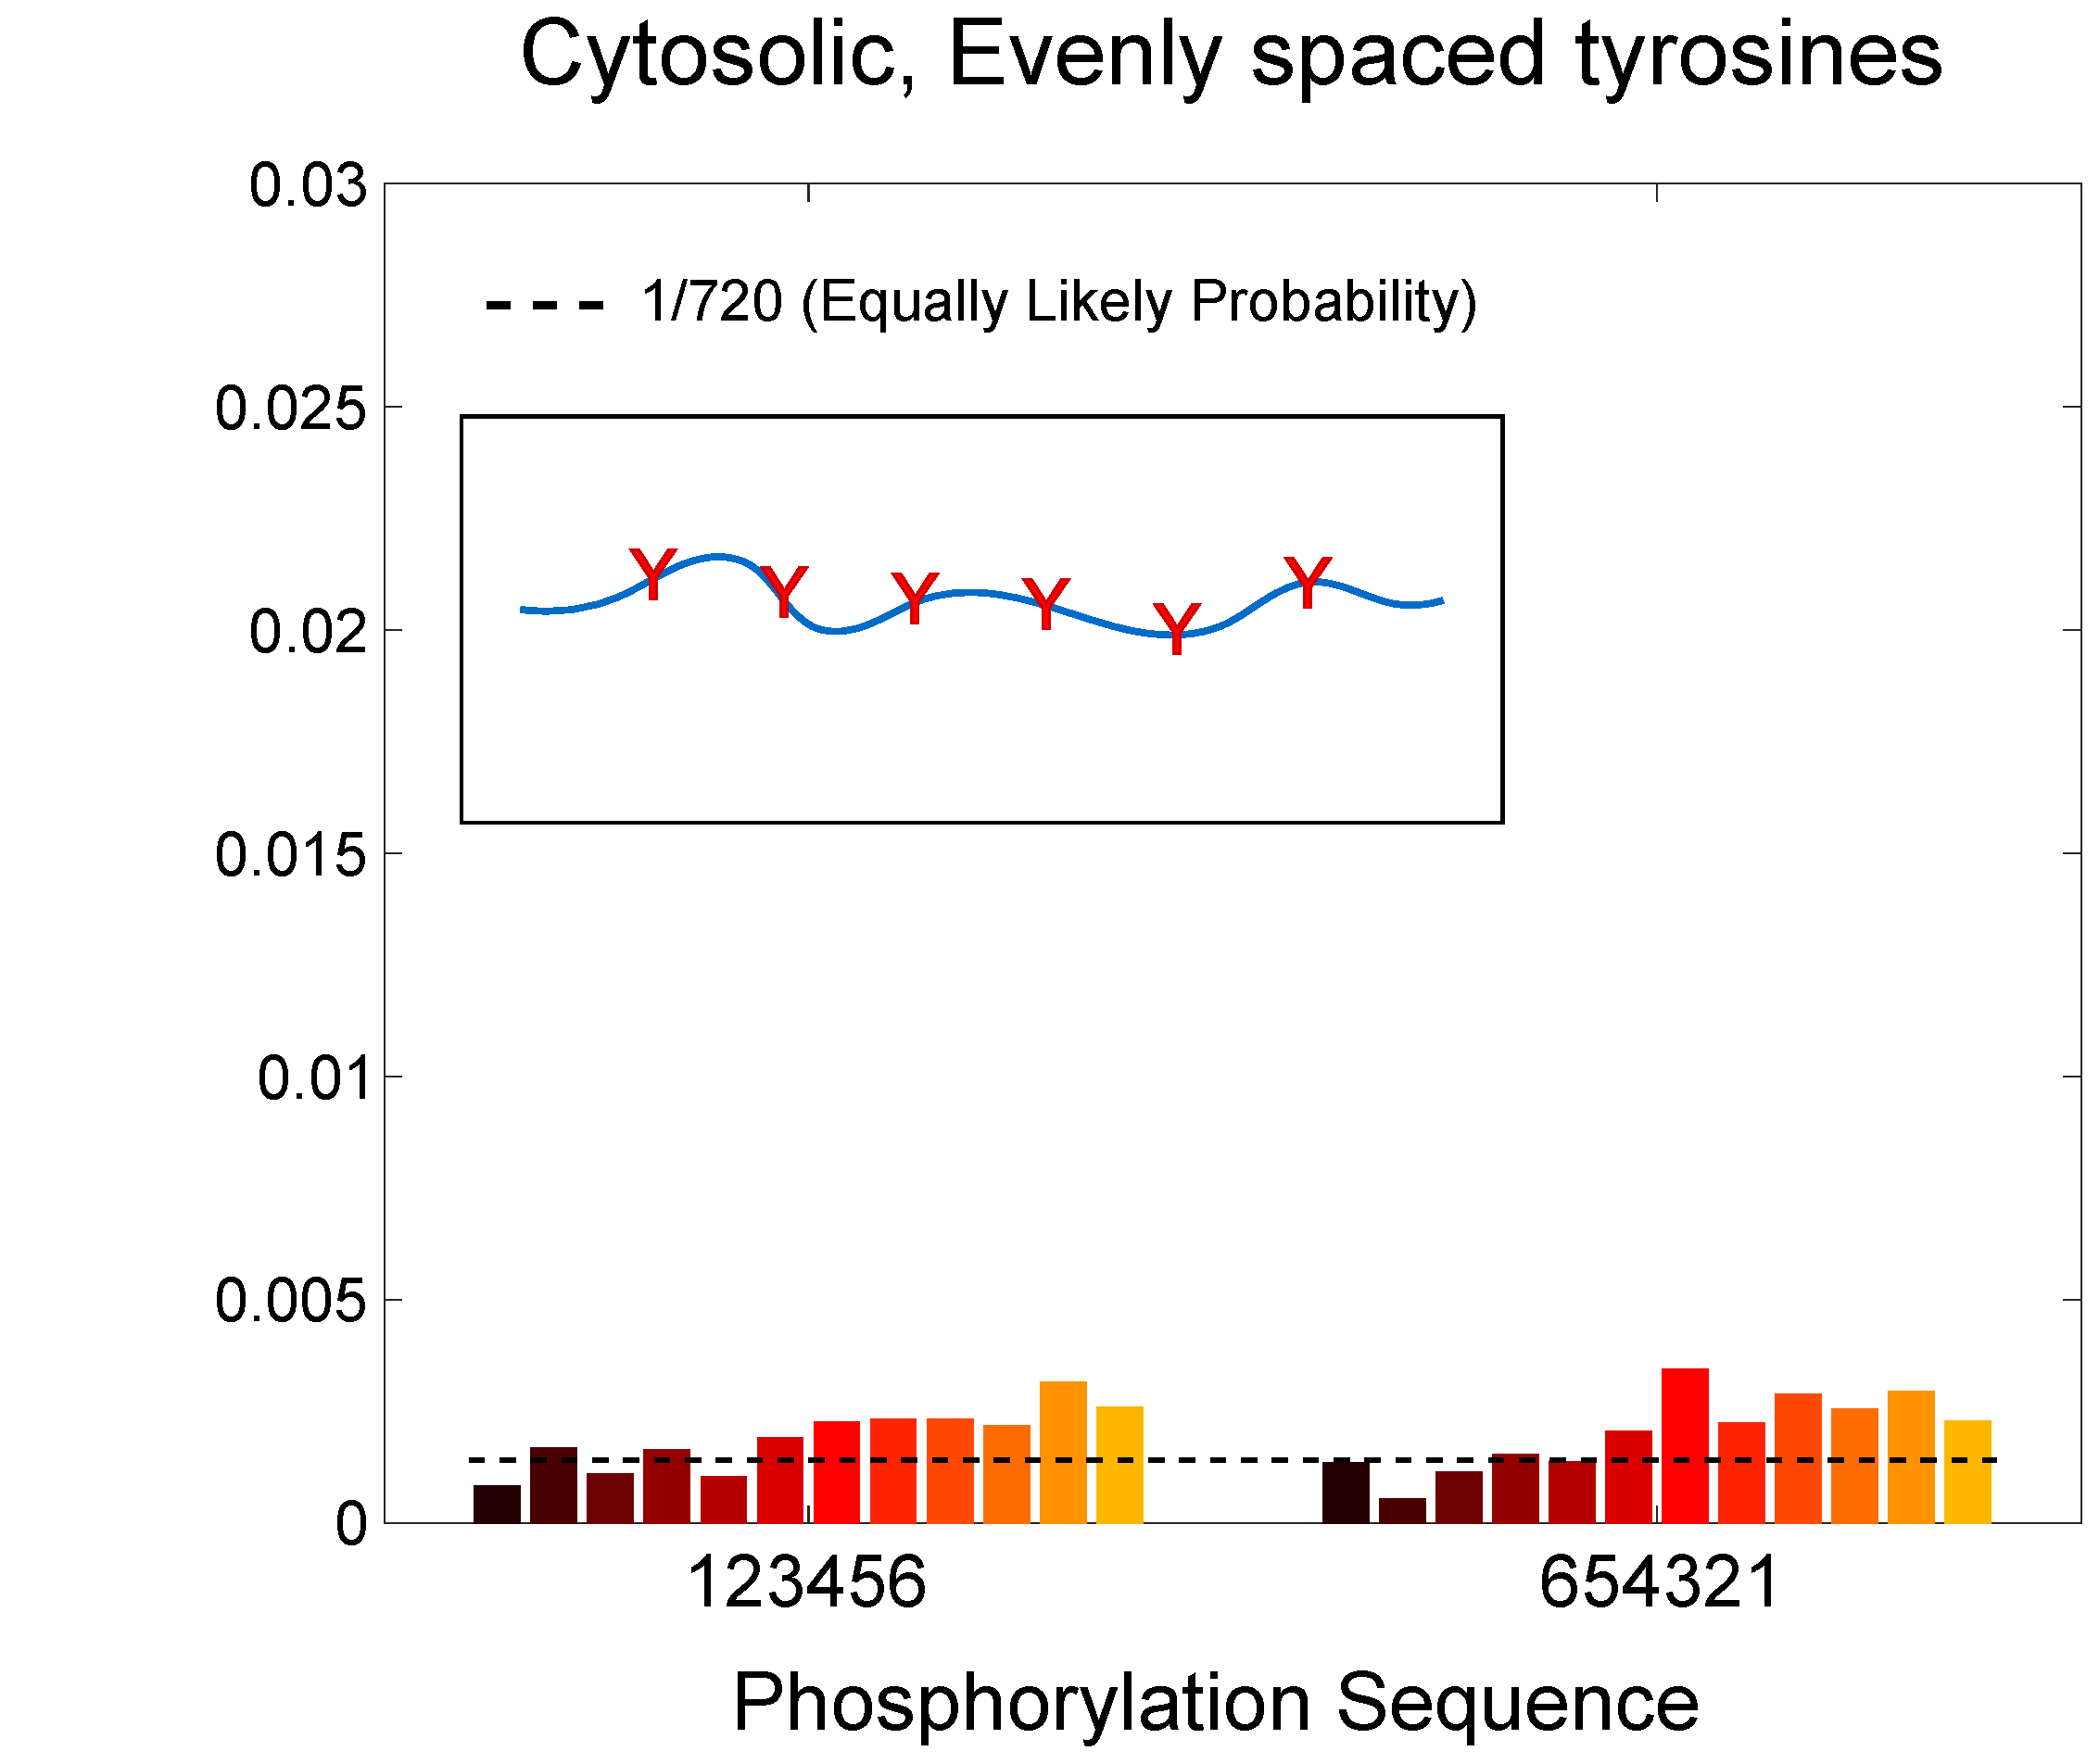
\includegraphics[width=\linewidth]{ResultsFigures/StiffeningSequentialBinding/EvenSites/ProbVSSequence.eps}
			\caption{}
		\end{subfigure}
	\end{center}
	\caption{Probability of phosphorylating membrane proximal to distal (123456) compared with distal to proximal (654321). Equally likely probability of all paths indicated with black, dotted line. (a) CD3$\zeta$ parameters, with membrane. (b) CD3$\zeta$ parameters, without membrane. (c) CD3$\zeta$ length, evenly spaced tyrosine locations, without membrane. }
\end{figure}


Presence of a membrane inherently leads to sequential binding, a feature that plays a key role in creating or enhancing ultrasensitivity.\hl{cite}



%%%%%%%%%%%%%%%%%%%%%%%%%%%%%%%%%%%%%%%%%%%%%%%%%%%
\subsection{Electrostatics}
%%%%%%%%%%%%%%%%%%%%%%%%%%%%%%%%%%%%%%%%%%%%%%%%%%%

\subsubsection{Introduction}

Subunits of many receptors have been shown to associate with the membrane prior to signalling. \hl{Others?  Dobbins et al, Chenqi paper} Close association with the membrane inhibits ligands from binding to their target site. Several of these chains have been shown to dissociate from the membrane after the extracellular receptor receives a stimulus. \hl{cite cite} This mechanism may help prevent unwanted signaling. \hl{wording here is mediocre}

In particular, evidence shows (\hl{CITE CITE CITE - Chenqi etc}) that CD3$\zeta$ associates with the membrane prior to phosphorylation, sequestering the tyrosines in the bilayer. Post-phosphorylation, CD3$\zeta$ is no longer associated with the membrane, but remains anchored by its transmembrane region. \hl{Is this true without stimulus?} \hl{what about stimulus without phosphorylation}

Additionally, basic residue regions in the CD3$\zeta$ and $\epsilon$ chains play a major role in maintaining the association between the polymer and the membrane. Studies show that mutation of the basic residue regions is sufficient to cause the protein to dissociate from the membrane.\hl{cite} Fully phosphorylated tyrosines are also sufficient to pull the protein away from the membrane, even when basic residue regions are present. \hl{cite} 

When the \hl{segment about mystery of where first signalling comes from}

\hl{discuss clusters of TCR? future modeling question?}

A molecular dynamics simulation of CD3$\epsilon$ indicates an approximately Gaussian distribution of the tyrosines, centered at the phospholipid heads of the membrane. \cite{Lopez2015}


\hl{evidence that fall off as feedback effect?} Although the tyrosines will spend much of their time sequestered in the membrane, there is some probability of entropic forces \hl{ehhh} transiently pulling them to the cytoplasm. \hl{hence distribution above....} When this occurs, Lck would be able to phosphorylate the tyrosine, creating a large negative charge on the chain. This phosphotyrosine would therefore repel the negative polar heads of the membrane, making it more favorable for that section of the polymer to pull out of the membrane.  

We hypothesize that since there is some probability for this first event to occur, then after the first event there would be a cooperative enhancement of the probability of neighboring tyrosines becoming accessible.  \hl{wording is terrible}

\hl{hypothesis about sequential binding?}

We model the polymer-membrane association as a potential acting on each rod in a freely-jointed chain in half space. The potential only acts in the direction of the half space plane (in this case, z-direction). To develop the model, we need to explore parameter space to create potentials which display the same behaviors seen experimentally and through molecular dynamics. In particular, we want to match three conditions:

\begin{enumerate}
	\item The polymer should display locational distributions consistent with Lopez et al. 2015. \cite{Lopez2015}
	\item When basic residues are mutated, the polymer should dissociate from the membrane.
	\item When all tyrosines are phosphorylated, the polymer should dissociate from the membrane.
\end{enumerate}

Based on these goals, we group residues into four distinct categories: tyrosines, phosphotyrosines, basic residues, and remaining residues. Based on these groups, we develop a set of possible relationships to explore (Table).  

\begin{table}[H]
\caption{Notation for electrostatic potentials applied to different groups of residues.}
\begin{center}
\begin{tabular}{ c | c}
\hline
Residue Group & Electrostatic Potential Abbreviation \\
\hline
Tyrosines & $E_Y$ \\
Phosphotyrosines & $E_P$ \\
Basic Residues & $E_B$ \\
Remaining Residies & $E_R$ \\
\hline
\end{tabular}
\end{center}
\end{table}

\begin{table}[H]
\caption{Electrostatic potential relationships to explore for behavior matching experimental results.}
\begin{center}
\begin{tabular}{| c | c |}
\hline
Group Number & Electrostatic Potential Relationship \\
\hline
\multicolumn{1}{|c|}{\multirow{2}[0]{*}{1}}  &  $E_Y = E_B < 0$\\
							&	   $E_P = E_R = 0 $\\
\hline
\multicolumn{1}{|c|}{\multirow{4}[0]{*}{2}}  &  $E_Y \neq E_B $\\
							&	   $E_Y < 0$ \\
							&	   $E_B < 0$ \\
							&	  $E_P = E_R = 0 $\\
\hline
\multicolumn{1}{|c|}{\multirow{5}[0]{*}{3}} 	& $E_Y \neq E_B$\\
							        & $E_Y < 0$ \\
								& $E_B < 0$ \\
								& $E_P > 0 $\\
								& $E_R = 0 $\\
\hline
\multicolumn{1}{|c|}{\multirow{3}[0]{*}{4}} 	& $E_Y = E_B <0 $\\
								& $E_P > 0 $\\
								& $E_R = 0 $\\
\hline
\multicolumn{1}{|c|}{\multirow{3}[0]{*}{5}} 	& $E_B <0 $\\
								& $E_Y = E_R=0 $\\
								& $E_P > 0 $\\
\hline
\end{tabular}
\end{center}
\end{table}					



%%%% Table of sequences and basic residues %%%%%%%

\begin{table}[H]
    \caption{Cytoplasmic amino acid sequence of CD3$\zeta$ and $\epsilon$ chains.  Basic residues (arginine, lysine, histidine) and tyrosines are highlighted separately in sequence.  Relative numeric location in cytoplasmic sequence and fraction of residues from that group are noted.}
    \begin{center}
    \begin{tabular}{|c|p{2cm}|p{8cm}|p{3.5cm}|p{1.6cm}|}
    	\hline
	Chain 		& 		Group			&		Location in Cytoplasmic Sequence	&	Numeric Location		&		\# / Total	\\
	\hline
	
	
    	\multicolumn{1}{|c|}{\multirow{2}[0]{*}{CD3$\zeta$}} 	&  	Basic Residues				& 	
	
	\hl{R}A\hl{K}FS\hl{R}SAETAANLQDPNQLYNELNLG\hl{RR}
	EEYDVLE\hl{KKR}A\hl{R}DPEMGG\hl{K}QQ\hl{RRR}NPQE
	GVYNALQ\hl{K}D\hl{K}MAEAYSEIGT\hl{K}GE\hl{RRR}
	G\hl{K}GHDGLYQGLSTAT\hl{K}DTYDAL\hl{H}MQTLAP\hl{R}			& 	
	
	1,3,5,28,29,37,38,
	39,41,48,51,52,53,60,65,
	67,72,78,81,82,83,85,91,
	99,102,106,113 		& 	
	
	29/113	\\
	\cline{2-5}
	
	
	
		&	 Tyrosines									&	
	
	RAKFSRSAETAANLQDPNQL\hl{Y}NELNLGRR
	EE\hl{Y}DVLEKKRARDPEMGGKQQRRRNPQE
	GV\hl{Y}NALQKDKMAEA\hl{Y}SEIGTKGERRR
	GKGHDGL\hl{Y}QGLSTATKDT\hl{Y}DALHMQTLAPR 				& 	
	
	21,32,60,72,91,102											&	
	
	6/113			\\
	\hline
	
	
	\multicolumn{1}{|c|}{\multirow{2}{*}{CD3$\epsilon$}}	&	 Basics Residues		&
	
	WS\hl{K}N\hl{RK}A\hl{K}A\hl{K}PVT\hl{R}GAGAGG\hl{R}Q\hl{R}GQN\hl{K}E\hl{R}
	PPPVPNPDYEPI\hl{RK}GQ\hl{R}DLYSGLNQ\hl{RR}I					& 	
	
	3,5,6,8,10,14,21,23,27,
	29,42,43,46,55,56	&		
	
	15/57	\\
	\cline{2-5}
	
	
		&		 Tyrosines				& 	
	
	WSKNRKAKAKPVTRGAGAGGRQRGQNKER
	PPPVPNPD\hl{Y}EPIRKGQRDL\hl{Y}SGLNQRRI			&
	
	 38,49		& 		
	 
	 2/57			\\
	\hline
    \end{tabular}
    \end{center}
\end{table}

\begin{figure}[H]
\begin{center}
    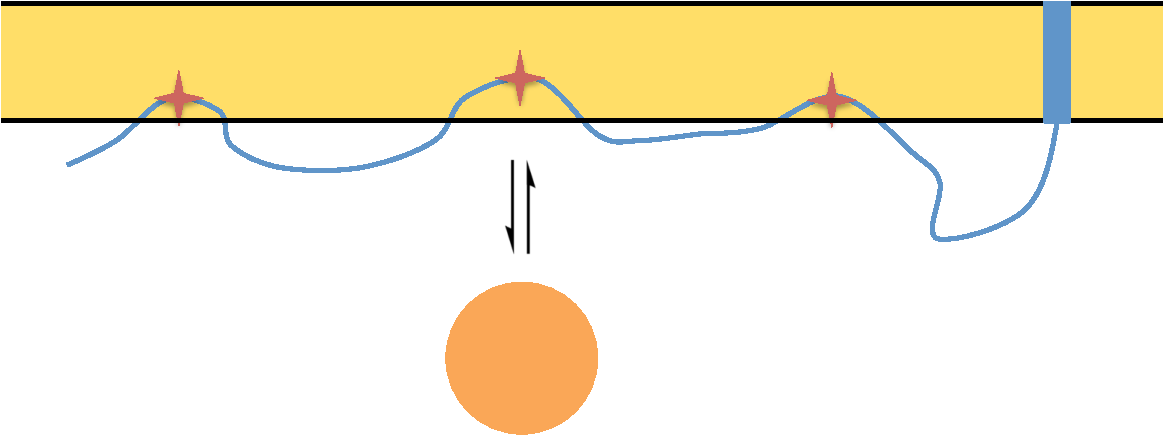
\includegraphics[width=0.7\linewidth]{ElectrostaticsDiagram.pdf}
    \caption{Cartoon of electrostatics model.  \hl{COULD HAVE POTENTIAL IN CARTOON?}. FJC associates with membrane, burying modification sites within membrane rendering them inaccessible to ligands.}
    \end{center}
\end{figure}

%%%%%%%%%%%%%%%%%%%%%%%%%%%%%%%%%%%%%%%%%%%
\subsubsection{Electrostatic Potentials}

There are many more basic residues compared to tyrosines in both the CD3$\zeta$ and $\epsilon$ chains.  Therefore, in order to account for tyrosine phosphorylation being sufficient to dissociate the polymer from the membrane, we would expect a repulsive force from the phosphorylated tyrosines. This directs our focus to Groups 3,4, and 5. Of these, we wish to look at the simplest cases first.  Therefore we consider the case where tyrosines do not experience their own potential but experience the potential of either the basic residues or experience the same potential as the rest of the amino acids.  Since tyrosines are not positively charged, it seems less likely that they would experience the same force as the basic residues.  Although their aromatic ring structure may help to anchor the polymer to the membrane once associated with the membrane, it would not drive the polymer to the membrane to begin with. \cite{Lopez2015} Therefore we focus initial efforts on Group 5.

\hl{It's possible I didn't need any of the above about different groups......`results not process' idea.}

There are many types of electric potential we could explore for the correct behavior.  Given that one of the phenomenons we wish to match is an approximately Gaussian distribution of both the tyrosines and polymer along the membrane edge, we use a parabolic-constant piecewise potential for our basic residues, instead of a Lennard-Jones potential.

Parabolic-constant piecewise potential:

Piecewise potential (aka, parabola-constant), ($PC$):
\begin{equation*}
\begin{cases}
width*z^2-depth 	& z<\sqrt{\frac{depth}{width}}\\
0 & z \geq \sqrt{\frac{depth}{width}} \\
\end{cases}
\end{equation*}

We have two possible potentials for the remaining amino acids.  In general, the peptide should not be able to penetrate deep into the membrane. Therefore, we can implement a hardwall or softwall constraint. The hardwall will prevent the remaining amino acids from passing the beginning of the membrane. A softwall constraint will allow amino acids to enter the membrane, but will incur an energetic penalty. 

Hardwall:

\begin{equation}
\begin{cases}
\infty 	& z < 0\\
0 & z \geq 0 \\
\end{cases}
\end{equation}


Softwall:

\begin{equation}
\begin{cases}
k*z^2 	& z < 0\\
0 & z \geq 0 \\
\end{cases}
\end{equation}



For the phosphorylated tyrosines, we will include an exponential distribution where the repulsive effect of the membrane drops off quickly as the phosphotyrosines move further away from the membrane.


Exponential decay:

\hl{go find actual equation to put here}

\begin{equation}
\begin{cases}
\infty	& z \leq 0\\
e^{-z} & z > 0 \\
\end{cases}
\end{equation}

\subsubsection{Initial Parameter Exploration}

We initially want to match the distribution of the polymer to the molecular dynamics simulations from Lopez et al. We sweep through parameters for the basic residue potential and the softwall potential. The softwall potential permits a Gaussian curve for the tyrosine distributions.  The hardwall condition \hl{(not shown)} prevents the distributions from spreading below the zero axis where we have defined the membrane to be. When we explore these parameters, multiple possibilities for parameter sets emerge which meet the distribution conditions. Below are examples of distributions arising from our parameter exploration for both a tyrosine and a basic residue. We note that the potentials affect the distribution of the basic residues more strongly than they affect the distributions of the tyrosines. From these parameter sets, we may refine our parameter search and begin exploring how the distributions are affected when all tyrosines are phosphorylated. 

\begin{figure}[H]
	\begin{center}
		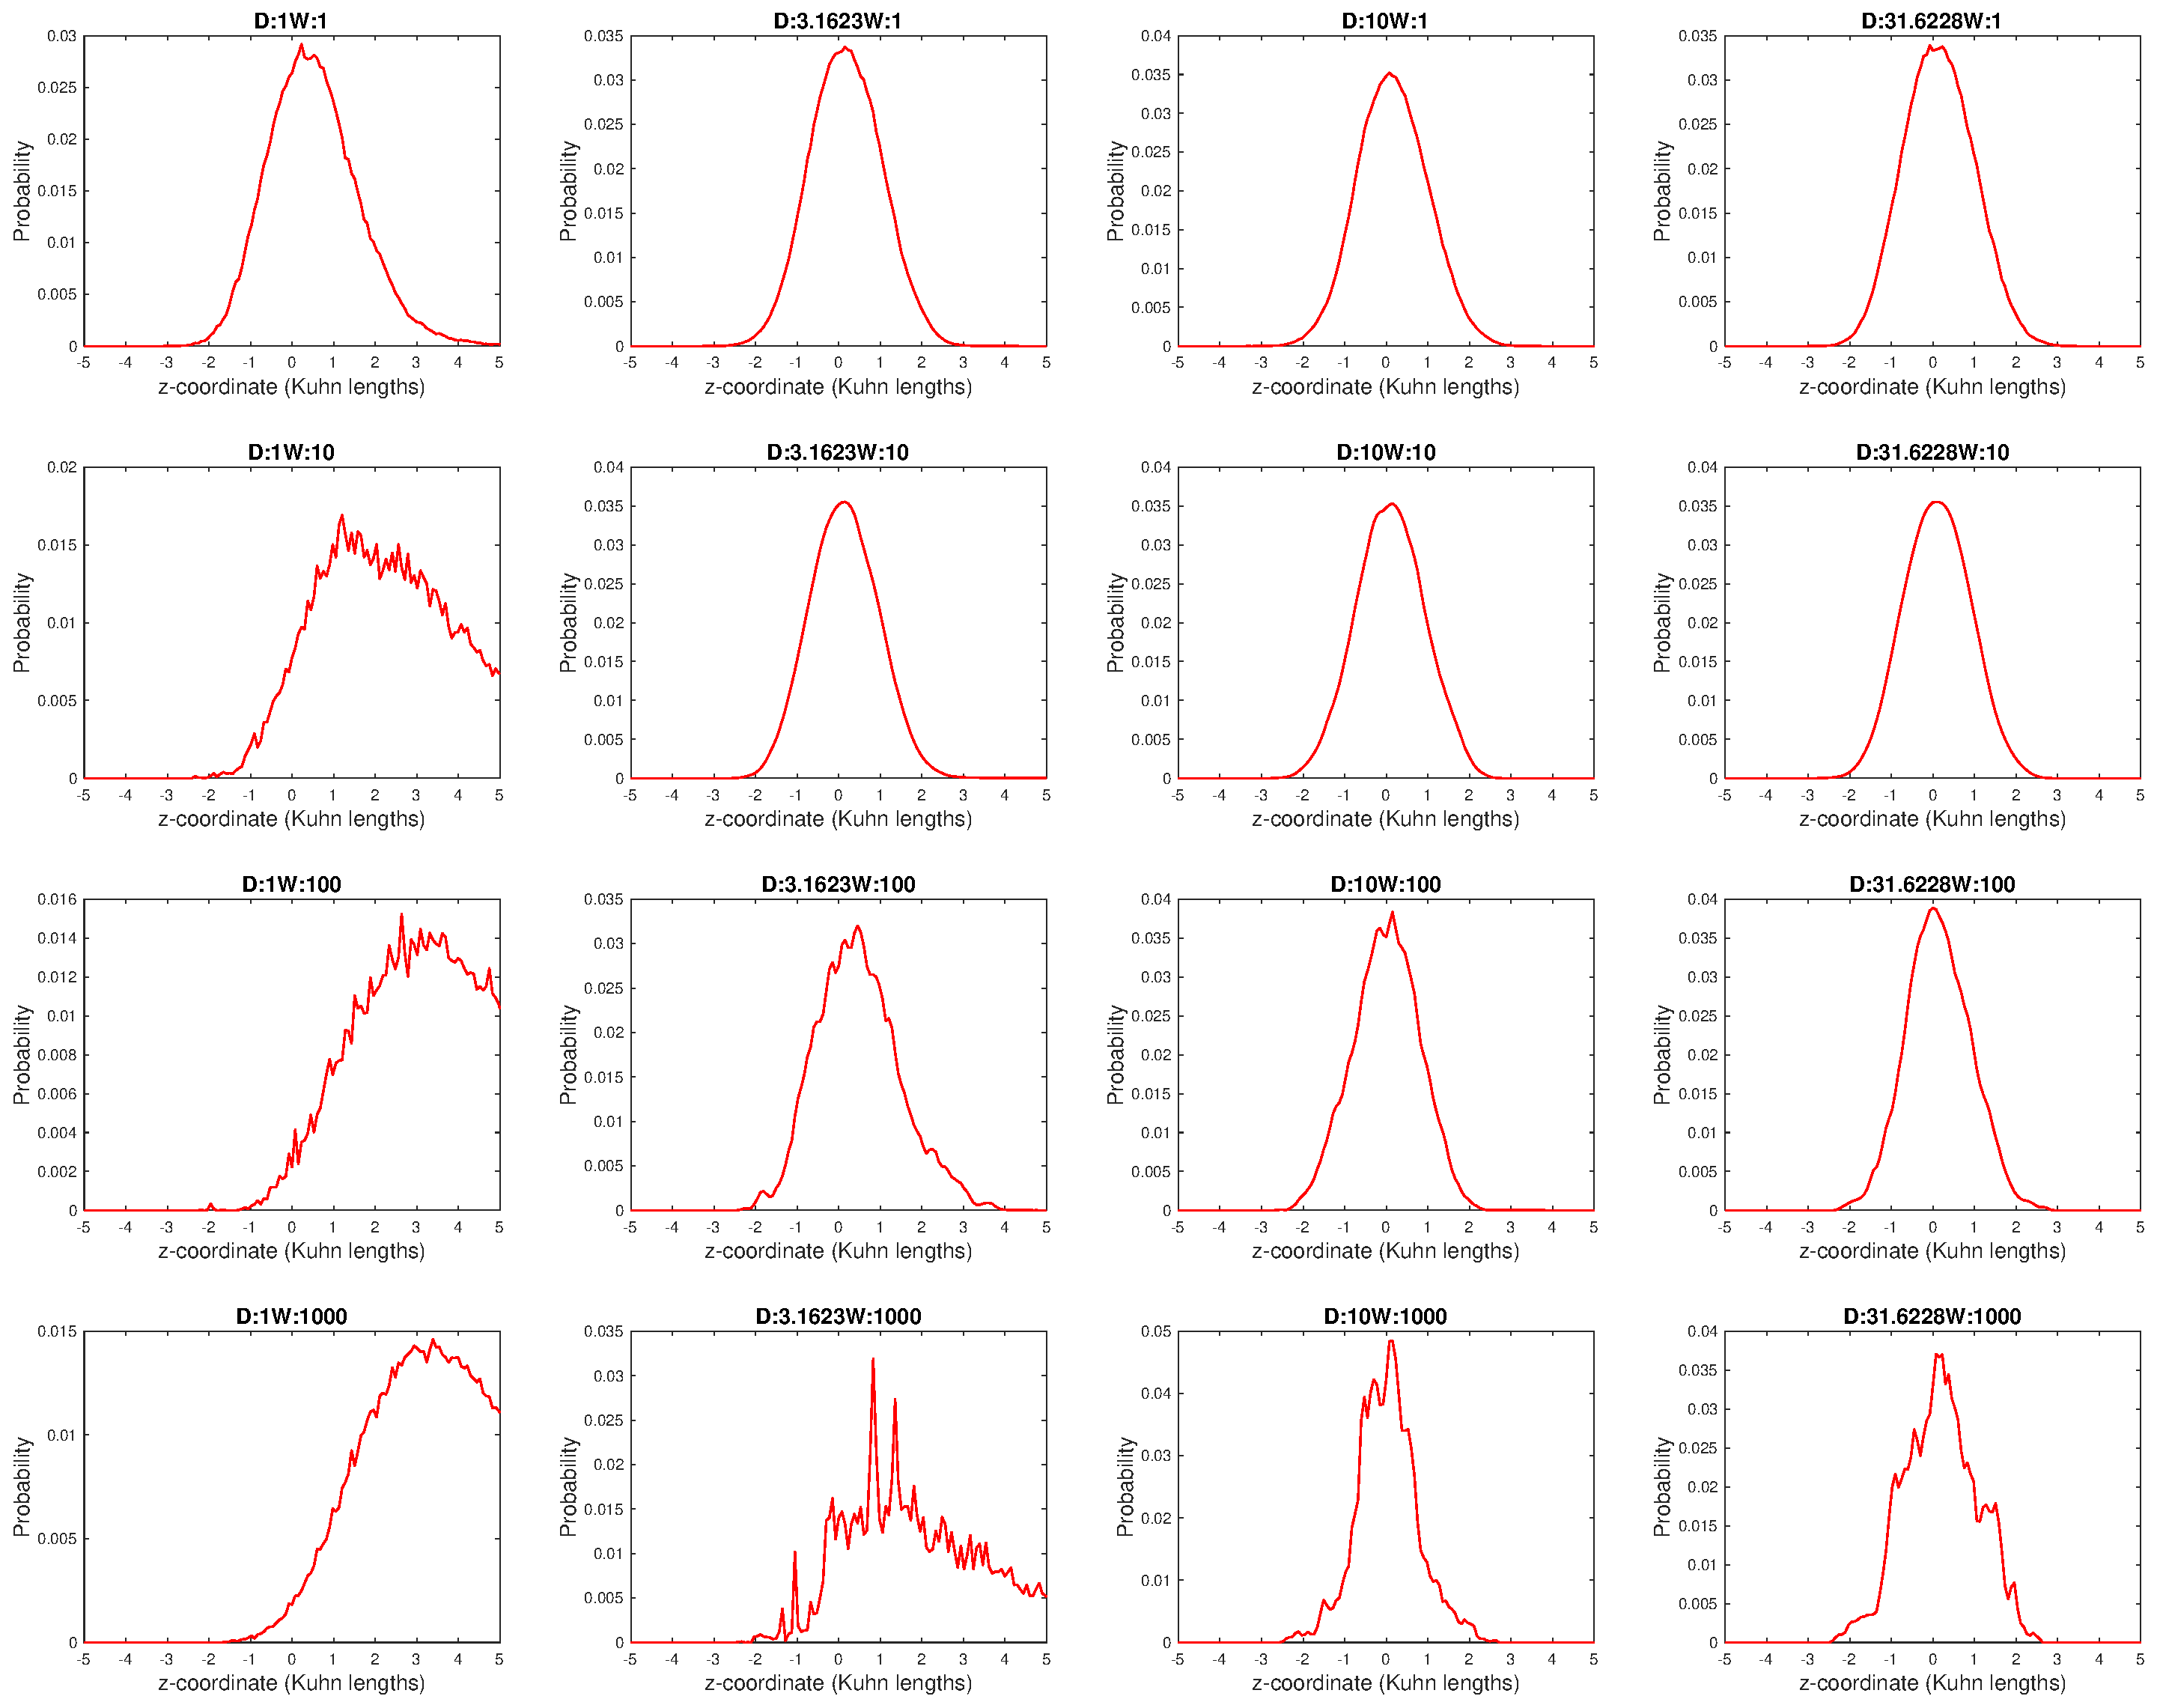
\includegraphics[width=0.8\linewidth]{ResultsFigures/Electro/DistributioniSite2.eps}
	\end{center}
	\caption{Tyrosine distribution resulting from parameter exploration of electric potentials. For this set, softwall potential is set at k=0.1. Basic residue potential depth ranges from $10^0$ to $10^{1.5}$.}
\end{figure}

\begin{figure}[H]
	\begin{center}
		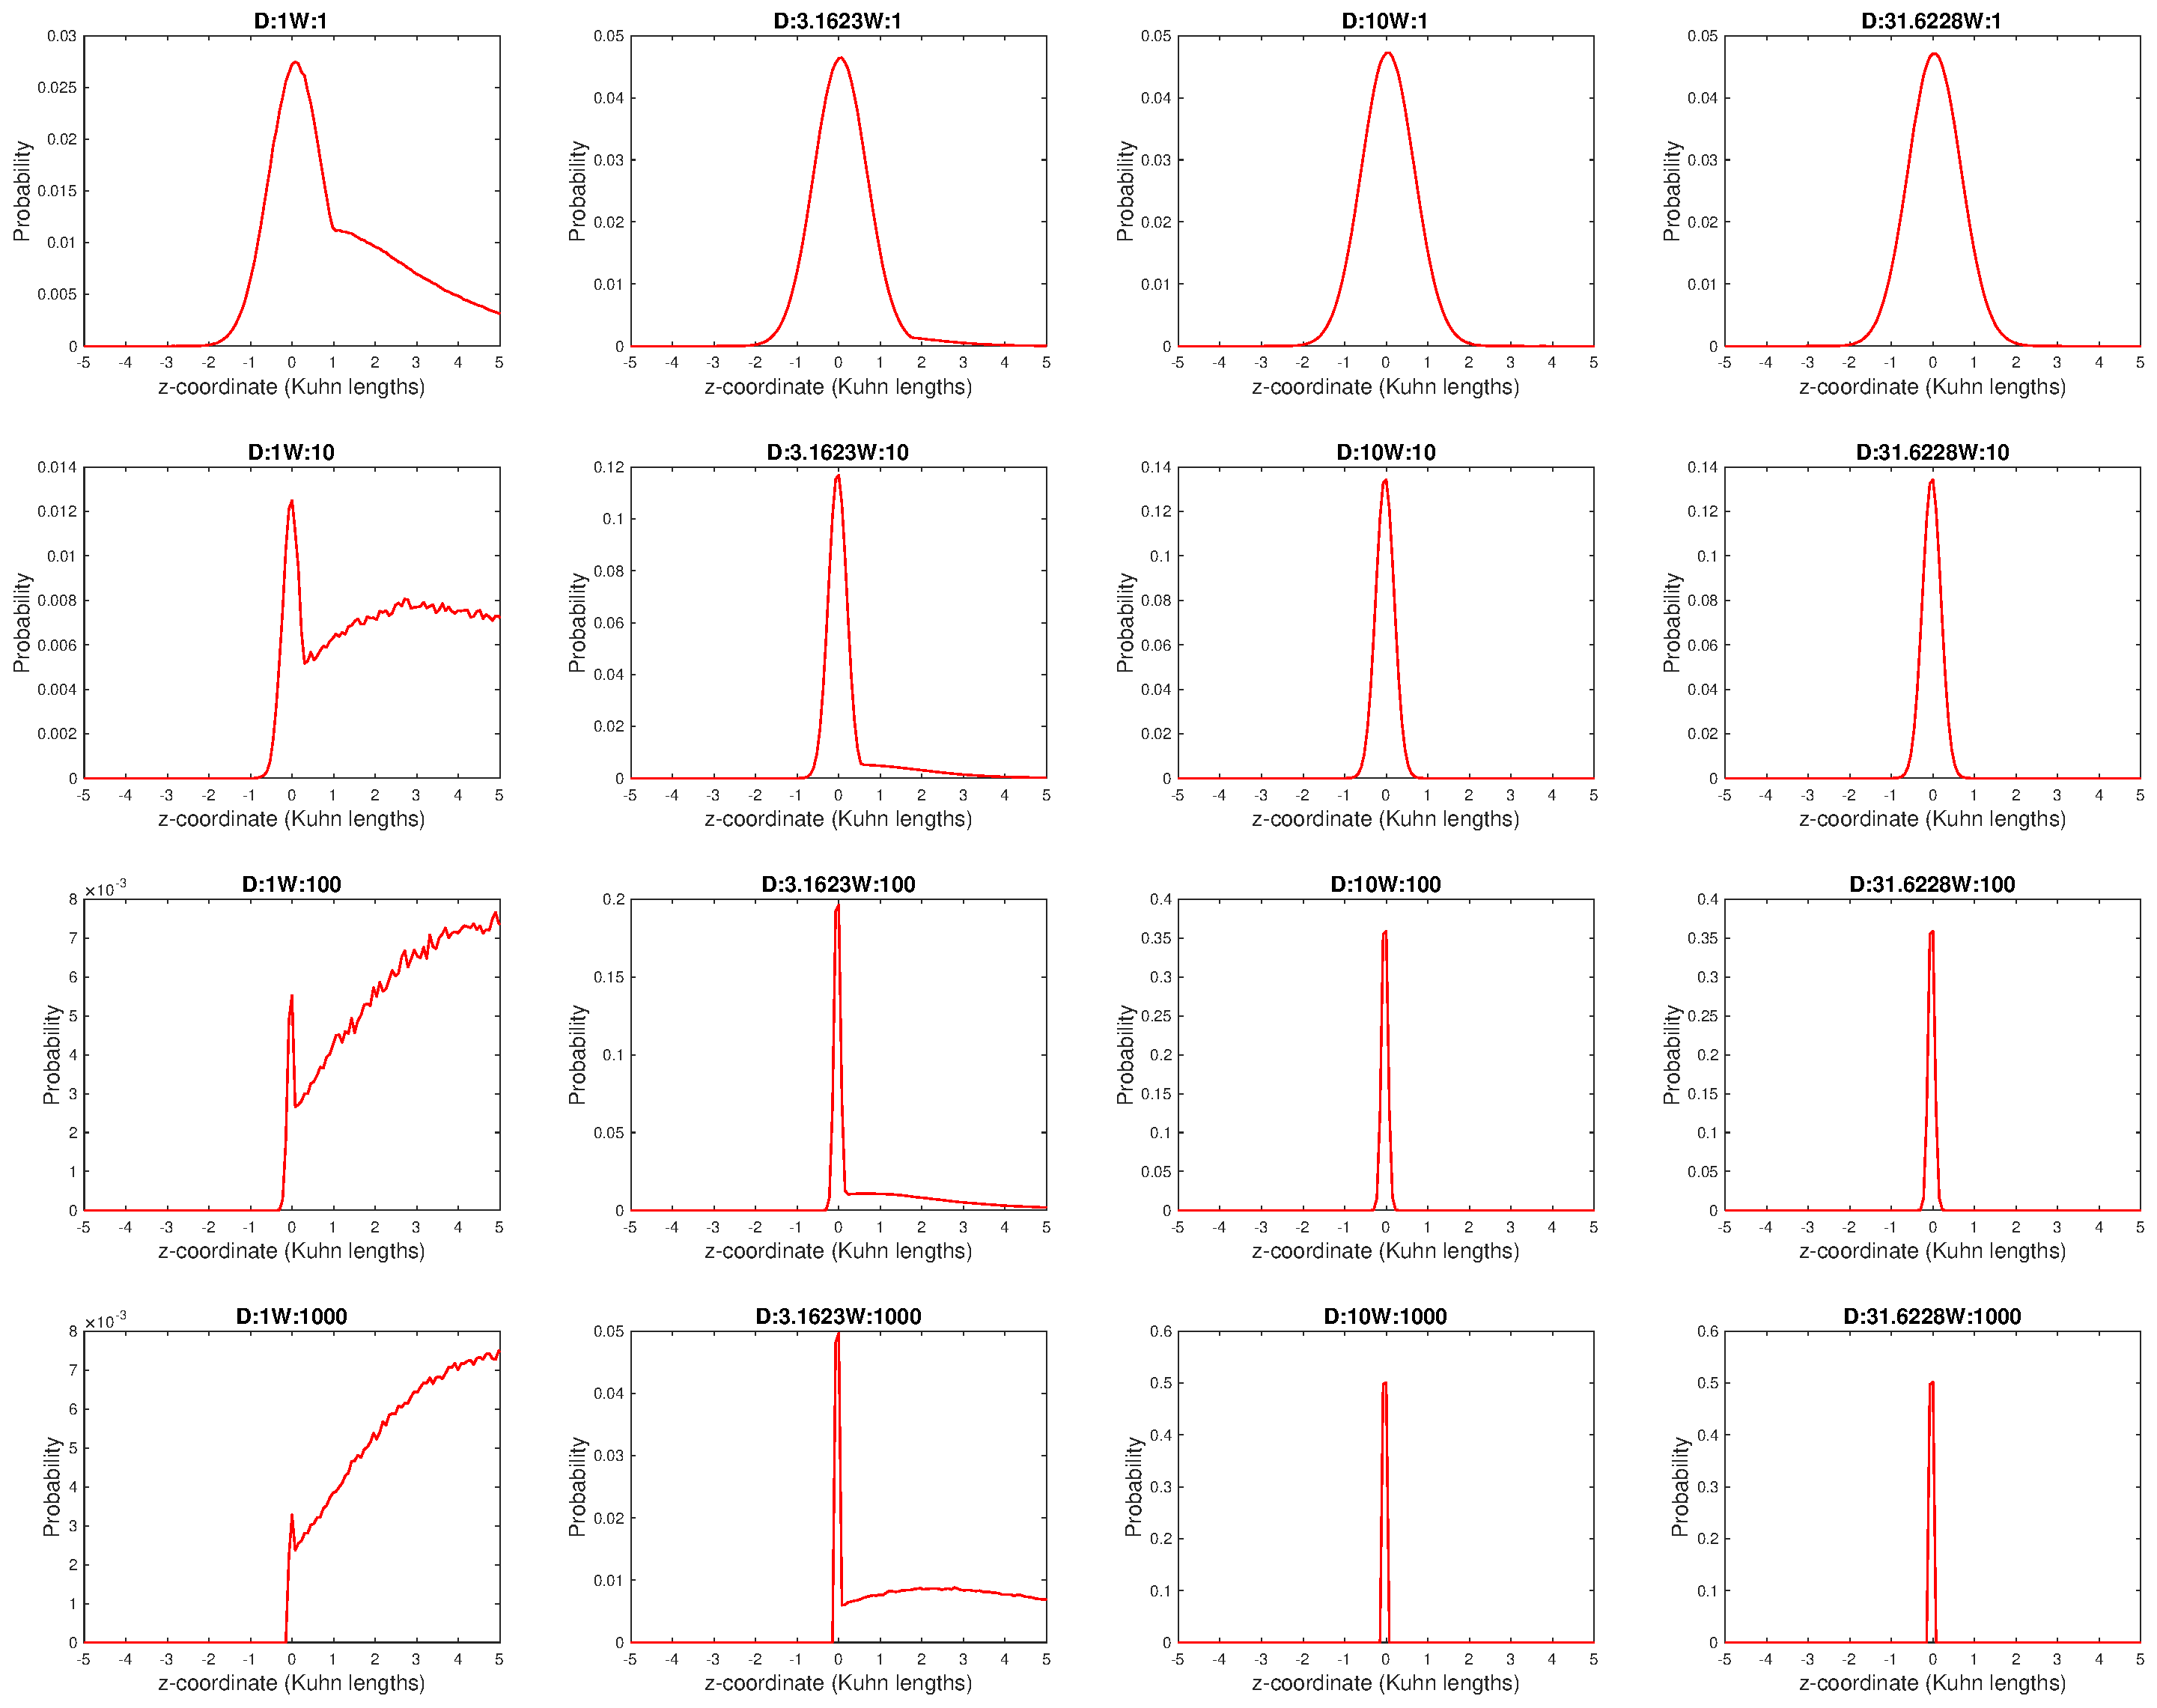
\includegraphics[width=0.8\linewidth]{ResultsFigures/Electro/DistributioniSite7.eps}
	\end{center}
	\caption{Basic residue distribution resulting from parameter exploration of electric potentials. For this set, softwall potential is set at k=0.1. Basic residue potential depth ranges from $10^0$ to $10^{1.5}$.}
\end{figure}




\subsubsection{Future Work}

First, we want to establish parameters (if they exist) which make our model exhibit the same behaviors as experimental and MD results. In particular, we now need parameters allowing the polymer to be free from the membrane when all tyrosines are phosphorylated. Either there will be only one reasonable parameter set which we can explore or there will be many parameter sets which display the desired properties.  If there are multiple parameter sets then we may try to find other experimental results to narrow our parameter regime. Alternatively, we may explore two or three major parameter regimes: weakest, strongest, and median potentials. The results from a wide spread of parameters will give us an indication of how much the parameters matter to the qualitative results.  

Second, with our parameter sets, we will now explore the effect of phosphorylation on the accessibility of successive tyrosines to a kinase.  We wish to see if there is a cooperative enhancement of the binding rates based on phosphorylation of previous residues.  Additionally, we will use this data to explore if there is a natural sequential binding sequence that arises.  One would imagine that once a single tyrosine is phosphorylated then its nearest neighbor would be the most likely next target.  However it is unclear if there is a first tyrosine that will be most likely to be phosphorylated and whether this will depend dominantly on basic residue distribution or on proximity to the transmembrane region.

\hl{paragraph about relating back to something useful or experimental?}

% potentially add image of mathematica plot to illustrate point


%%%%%%%%%%%%%%%%%%%%%%%%%%%%%%%%%%%%%%%%%%%%%%%%%%%
\end{document}
%%%%%%%%%%%%%%%%%%%%%%%%%%%%%%%%%%%%%%%%%%%%%%%%%%%





